\documentclass[a4paper, 12pt, %
draft,%
pdftex]{report} % make report->book for two sided final publishing.
\fussy
\sloppy

\usepackage{upthesis}
% Cause floats to always be below  where they are inserted as per
% Prof. de Vaal.
% \usepackage{flafter}
\usepackage{fancybox}
\usepackage{pgf}
\usepackage{pgfplots}
\usepackage{sparklines}
\usepackage{microtype}
\newcommand{\citehere}{\fbox{\bf Citation needed!}}
\newcommand{\num}[1]{\ensuremath{\fnum{#1}}}
\newcommand{\units}[1]{\ensuremath{\mathrm{#1}}}
\newcommand{\xxx}{\fbox{\bf XX Check XX}}

\newcommand{\prob}[1]{\ensuremath{\mathrm{P}(#1)}} % probability of event
\newcommand{\expect}[1]{\ensuremath{\mathrm{E}(#1)}} % Expectation of variable

% TODO: Typeset different code modules seperately, reference code documentation!
\newcommand{\modulename}[2]{{\tiny #1}\fbox{#2}} % typeset module name - language, modulename

% Title and author definitions
\title{Generic Framework for Chemical Process Modelling with Stochastic Inputs} 
\author{Carl Sandrock} 
\degree{Philosophiae Doctor (Control Engineering)} 
\department{Department of Chemical Engineering} 
\date{November 2010}

% Include directives
\includeonly{
front,
% -- Text Starts --
introduction,
statistics,
optimisation,
flowsheeting,
segmentation,
montecarlo,
software,
design,
testproblems,
implementation,
results,
conclusion,
% -- Appendix Entries --
%programmingdetails,
% -- Back matter --
back
}

\begin{document}

\maketitle
\makecoverpage

\pagestyle{plain}
\thispagestyle{plain}
\pagenumbering{roman}

\chapter*{Synopsis}\addcontentsline{toc}{section}{Synopsis}

Chemical engineering process modelling and simulation pose significant challenges to the computer program developer.
Chemical processes are invariably described by non-linear equations such as chemical reaction kinetics, flow-pressure relationships and physical properties.
Dynamic simulation of such systems involves the solution of sets of non-linear differential and algebraic equations.
There is also uncertainty associated with the model equations themselves (model uncertainty), their parameters (parametric uncertainty) and the inputs into the model (input uncertainty).
Tools that aid chemical engineers in the solution of these problems have been successfully commercialised and enjoy a measure of success, although the adoption of dynamic and stochastic simulation packages is lagging behind the steady-state flowsheeting tools.

Commercial software solutions can be prohibitively expensive in addition to confining users to adhere to proprietary standards.
 The Free Software and Open Source movements have made inroads into providing non-proprietary alternatives to many commercial software packages, which has encouraged the adoption of open standards.
 Pressure from the commercial users of simulation software also led to the development of the CAPE-Open standards to ensure interoperability between proprietary platforms.

This work presents a framework for the development of stochastic dynamic simulations of chemical processes using only free and open source software.
 The large problem of stochastic dynamic simulation has been broken down into stages:
\begin{enumerate}
\item Input modelling using Markov chain models trained on process data or seeded by hand in addition to stationary distribution models. This enables dynamic scenarios to be handled with the minimum of special case code generation.
\item Process modelling using an object-oriented approach in the Modelica language. Modelica has an open source implementation called OpenModelica and is an open standard modelling language.
\item Monte Carlo simulation using extensions to the OpenModelica compiler that ease parallel simulations
\item Postprocessing, including visualisation and statistical analysis. Statistics that are generated can be used for control or validation purposes.
\end{enumerate}

\noindent \textbf{KEYWORDS:} 

\begin{otherlanguage}{afrikaans}
\chapter*{Sinopsis}\addcontentsline{toc}{section}{Sinopsis}
%TODO: reTranslate (current one by google translate)
Chemiese ingenieurswese proses modellering en simulasie inhou groot uitdagings aan die rekenaar program ontwikkelaar. 
Chemiese prosesse is altyd beskryf deur nie-line�re vergelykings soos chemiese reaksie kinetika, vloei-druk verhoudings en fisiese eienskappe. 
Dinamiese simulasie van sodanige stelsels behels die oplossing van stelle van nie-line�re differensiaal-en algebra�ese vergelykings. 
Daar is ook onsekerheid in verband met die model vergelykings hulself (model onsekerheid), hul parameters (parametriese onsekerheid) en die insette in die model (insette onsekerheid). 
Instrumente wat steun chemiese ingenieurs in die oplossing van hierdie probleme suksesvol is gekommersialiseer en geniet 'n mate van sukses, hoewel die aanneming van' n dinamiese en stogastiese simulasie pakkette is agter die stabiele toestand flowsheeting tools. 

Kommersi�le sagteware oplossings kan word onbetaalbaar bykomend tot beperk gebruikers om te voldoen aan eie standaarde. 
 Die Vrye Sagteware en Open Source bewegings het het vordering in die verskaffing van nie-eie alternatiewe vir baie kommersi�le sagteware pakkette, wat aangemoedig om die goedkeuring van oop standaarde. 
 Druk van die kommersi�le gebruikers van simulasie sagteware ook gelei tot die ontwikkeling van die Kaapse-Open standaarde interoperabiliteit te verseker tussen die eie platforms. 

Hierdie werk bied 'n raamwerk vir die ontwikkeling van stogastiese dinamiese simulasies van chemiese net gratis en open source sagteware prosesse gebruik. 
Die groot probleem van stogastiese simulasie dinamiese is afgebreek in fases:
\begin{enumerate}
  \item Input modelle gebruik Markovketting modelle opgelei oor die proses data
   of gekeur per hand benewens stasion\^ere verdeling modelle. Dit stel
   dinamiese scenario's te hanteer word met die minimum van spesiale geval code generasie. 
  \item Prosesmodellering met behulp van 'n objek-geori�nteerde benadering in
  die Modelica taal. Modelica het 'n oop bron implementering genoem OpenModelica
  en is 'n oop standaard model taal.
  \item Monte Carlo-simulasie met uitbreidings aan die OpenModelica samesteller dat gemak parallel simulasies
  \item Post Processing, insluitend visualisering en statistiese analise.
  Statistiek wat gegenereer kan gebruik word vir die beheer of validering voorgel�.
\end{enumerate}

\bigskip 

\noindent \textbf{SLEUTELWOORDE:} 

\end{otherlanguage} 

% Local Variables: 
% TeX-master: "thesis" 
% End:



\chapter*{Acknowledgements}\addcontentsline{toc}{section}{Acknowledgements}

My parents, for encouraging me to continue with my education and
supplying a solid example of dedication to learning.  Ruanne, my
supportive wife: we can stop waiting now.  The numerous friends at the
University of Pretoria who have helped me to cope with my
procrastination and the stress of preparing this document.

\vfil

\begin{flushright}
  
\includegraphics[height=24pt]{penguin} 
  \shortstack{Typeset using \LaTeXe\ \\ 
    Compiled under GNU/Linux}
\end{flushright}

% Local Variables:
% TeX-master: "thesis"
% End:


\tableofcontents
\newpage
\listoffigures
\newpage
\listoftables
\newpage
%\chapter*{Nomenclature}
\printnomenclature
\newpage

% Local Variables:
% TeX-master: "thesis"
% End:


% Page numbering: Start at 1

\pagestyle{headings}
\setcounter{page}{1}
\pagenumbering{arabic}

\chapter{Introduction}\label{chap:intro}

Chemical engineering process modelling and simulation poses a
significant challenge to the computer program developer.  Chemical
processes are invariably described by nonlinear equations such as
chemical reaction kinetics, flow-pressure relationships and physical
properties.  Dynamic simulation such systems involves the solution of
sets of nonlinear differential and algebraic equations.  There is also
uncertainty associated with the model equations themselves (model
uncertainty), their parameters (parametric uncertainty) and the inputs
into the model (input uncertainty).

This work aims to present a framework for the development of
stochastic dynamic simulations of chemical processes.  The framework
is designed to be generic.  The large problem of stochastic dynamic
simulation has been broken down into three steps: input modelling,
process modelling and postprocessing.  

This document is divided into three sections

Each step of the simulation is
discussed


% Local Variables:
% TeX-master: "thesis"
% End:

\part{Literature}
\chapter{Flowsheeting}

\begin{overview}
  Even though many representations of chemical processes are possible
  in theory, the flowsheet is the most popular in practice.  Process
  engineers use process flow diagrams and piping and instrumentation
  diagrams to document processes and flowsheeting software leverages
  their familiarity with the flowsheet format to represent the
  processes being simulated.  An overview is given here of
  flowsheeting terminology and common unit operations, along with
  common methods of solving dynamic and stationary flowsheeting
  problems.
\end{overview}

\section{Unit operations}
The concept of unit operations has been embedded in Chemical
Engineers' psyche since Arthur D. Little coined the phrase in
1915~\citep{hougenhistory}.  Unit operations lend themselves to an
object-oriented programming style, with their main functions
encapsulated in a ``black box'', with narrow interfaces between them.
The following main unit operations are identified, following the
sequence used in~\citet{msh}.

\subsection{Fluid flow operations}
These operations are further subdivided based on the nature of the
fluid flowing in them.  Uncompressible and compressible single phase
flow are the most commonly modelled types; multiphase flow is commonly
encountered in industry, but presents significant modelling
challenges.\citehere.

\subsubsection{Fluid movers}
This category encapsulates pumps, blowers, compressors and similar
equipment which bring about a change in momentum of a fluid by doing
work on it.  

\subsubsection{Valves}


\subsubsection{Pipes}


\subsection{Heat transfer}
\subsubsection{Heat exchangers}


\subsection{VLE}
Mass transfer operations 


%% Mention something about the phase rule and degrees of freedom

\subsubsection{Flashing}
A flash drum is a unit that separates a stream into a vapour and
liquid fraction based on the difference in composition of vapour and
liquid in phase equilibrium.  Figure~\ref{fig:flashdrum} shows a flash
drum with the relevant variables.

\begin{figure}[htbp]
  \centering
  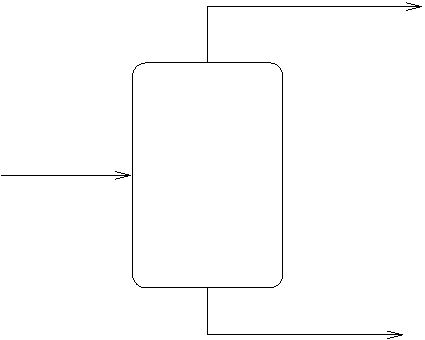
\includegraphics[width=0.4\textwidth]{flashdrum}
  \caption{Flash drum}
  \label{fig:flashdrum}
\end{figure}

The following assumptions are common when modelling flash drums:

\begin{itemize}
\item The phase equilibrium is achieved fully and quickly relative to
  the dynamics of the level of the flash drum.
\item The pressure in the flash drum changes only due to changes in
  the vapour balance.
\end{itemize}

Under these assumptions, the equations describing the dynamic
behaviour of a standard flash drum are given below (from \citet{eich-soellner_stationary_1997}):

\begin{align}
  \dxdy{M}{t} &= F - V - L \\
  \dxdy{M\vec{x}}{t} &= Fx_j - Vy_j - Lx_j \text{ for } j = 1,\dots,n_c-1  \\
  \sum_{j=1}^{n_c} x_j &= 1 \\
  \sum_{j=1}^{n_c} y_j &= 1 \\
  y_j &= K_j(T, P, x, y)x_j \text{ for } j = 1,\dots,n_c-1  \\
  L &= \Phi(M) \\
  \dxdy{Mh_L}{t} &= Fh_F - Vh_V - Lh_L + Q \\
  h_p &= h_p(T_p, P_p, x) \text{ for } i \in {L, V} \\
  P_V &= P_L = P
  T_V=T_L=T
\end{align}

\subsection{Distillation}

The vapour-liquid equilibrium-based separation obtained in a flash unit can be
repeated an arbitrary number of times to obtain better separation as
long as the equilibrium allows for enrichment of the vapour.  A
distillation column is an integrated system allowing for repeated
equilibrium stages.  Liquid flows down the column under the influence
of gravity and vapour flows upward due to the difference in density
between the vapour and the liquid.  The vapour contacts with the
liquid on plates or on the surface of a packing material.  

A plated column can be described by similar equations as the flash
drum unit already discussed, with some coupling between the plates.
The amount of liquid on a column plate is called the holdup.

The following needs to be taken into account:

The flow of liquid down the column is a hydraulic prolem, involving
the flow over a weir.  The Francis weir formula describes this flow.


\subsection{Chemical reaction operations}

\subsubsection{Stoicheometry}
Given a system of reactions such as:
\begin{equation}
  xA_iB_j -> yA_k + zB_lA_m,
\end{equation}
it is required that the reaction ``balances'', that is that the number
of atoms of A and B are unchanged by the reaction.  In the above case,
this implies that $xi=yk+zm$ and $xj=zl$.  It is usually desired to
find integer solutions for $x$, $y$ and $z$ given $i$ to $m$.  This is
known as balancing the reactions.  Once such solutions have been
found, they are known as the stoicheometric coefficients of the
reaction scheme.  It is useful to group the stoicheometric
coefficients into a stoicheometric matrix $\alpha$ such that the
magnitude of $\alpha_{i,j}$ is the coefficient of component $j$ in
equation $i$ ($x$ in the example above) and the sign of $\alpha_{i,j}$
is negative for reactants and positive for products.  Using this
notation, the following equations must hold at any time:
\begin{equation}
  \sum_{j=1}^{n_c} \alpha_{i,j}A_j = 0,~i=1,\dots,M
\end{equation}
Here, $A_j$ is the amount of component $j$ and $M$ is the  number
of reactions.

\subsubsection{Reaction rates}
Reaction rates are commonly modelled using the notation
$r_i=-\dxdy{C_i}{t}$, where $r_i$ is the reaction rate and $C_i$ is the
concentration of component $i$.  

Reaction rates are often given by a power law rate equation
\begin{equation}
  r_i = k_i \prod_{j=1}^{n_c}c_j^{\beta{i,j}} - k'_i\prod_{j=1}^{n_c}c_j^{\gamma{i,j}}
\end{equation}

The order 

\subsubsection{Rate constants}

\subsubsection{CSTR}

\section{Steady state}

% Local Variables:
% TeX-master: "thesis"
% End:


\chapter{Statistics and signal analysis}\label{chap:stats}
\begin{overview} 
  This chapter explores existing developments in modelling and
  simulating steady-state and dynamic systems with and without
  uncertainty.
\end{overview}

\section{Stationary statistics}

\section{Signal statistics}

\subsection{IEC 61131-3}
IEC 61131-3 is a standard that defines

\url{http://en.wikipedia.org/wiki/IEC_61131-3}

\section{Basic modelling equations}
Several equations are used in many different pieces of equipment
\subsection{Conservation of mass}
\subsection{Conservation of energy}
\subsection{Reaction kinetics}



\subsection{Equilibrium}
\subsection{Transport equations}
\subsubsection{Heat transfer}
\subsubsection{Mass transfer}

\section{Simulation}

\subsection{Modelling}
\subsubsection{Microscopic}

\subsubsection{Macroscopic}
Macroscopic modelling 

\subsubsection{Lumped models}

\subsection{Input identification}
Stochastic simulation of systems, especially those using Monte Carlo
methods, require good input scenarios to generate good output data.
It is common to make use of Markov processes to generate realistic
inputs based on historic data.  However, identification of ``events''
within historic data can be troublesome.  Much work has been done on
identification of events or trends in data (\citet{maurya.rengaswamy.ea2007fault}
give a good overview of trend analysis techniques).  Reducing process
signals to symbols representing qualitative event types rather than
quantitative data allows patterns to be found in events, or what
\citet{cheung.stephanopoulos1990representation} refer to as
episodes.  In this seminal work, the authors define a formal language
in terms of the 7 primitives shown in
figure~\ref{fig:stephanopoulosprimitives}.

\begin{figure}[htbp]
  \centering
  \setlength{\unitlength}{0.7em}
  {\small
  \begin{picture}(8,8)
    \put(0,0){\line(1,0){8}}
    \put(0,0){\line(0,1){8}}
    \put(7,1){D}
    \put(4,4){$(+,-)$}
    \thicklines
    \qbezier(1,1)(2,7)(7,7)
  \end{picture}
  }
  {\small
  \begin{picture}(8,8)
    \put(0,0){\line(1,0){8}}
    \put(0,0){\line(0,1){8}}
    \put(7,1){B}
    \put(1,4){$(+,+)$}
    \thicklines
    \qbezier(1,1)(7,2)(7,7)
  \end{picture}
  }
  {\small
  \begin{picture}(8,8)
    \put(0,0){\line(1,0){8}}
    \put(0,0){\line(0,1){8}}
    \thicklines
    \qbezier(1,1)(2,2)(7,7)
    \put(7,1){C}
    \put(1,5){$(+,0)$}
  \end{picture}
  }
  {\small
  \begin{picture}(8,8)
    \put(0,0){\line(1,0){8}}
    \put(0,0){\line(0,1){8}}
    \thicklines
    \qbezier(1,7)(6,7)(6.7,1)
    \put(7,1){G}
    \put(1,4){$(-,-)$}
  \end{picture}
  }
  {\small
  \begin{picture}(8,8)
    \put(0,0){\line(1,0){8}}
    \put(0,0){\line(0,1){8}}
    \thicklines
    \qbezier(1,7)(2,2)(6.7,1)
    \put(7,1){E}
    \put(4,4){$(-,+)$}
  \end{picture}
  }
  {\small
  \begin{picture}(8,8)
    \put(0,0){\line(1,0){8}}
    \put(0,0){\line(0,1){8}}
    \thicklines
    \qbezier(1,7)(4,4)(7,1)
    \put(7,1){F}
    \put(5,5){$(+,-)$}
  \end{picture}
  }
  {\small
  \begin{picture}(8,8)
    \put(0,0){\line(1,0){8}}
    \put(0,0){\line(0,1){8}}
    \thicklines
    \qbezier(1,4)(3,4)(7,4)
    \put(7,1){A}
    \put(4,6){$(0,0)$}
  \end{picture}
  }
  \caption[Episodic analysis primitives]{Episodic analysis primitives according to \citet{cheung.stephanopoulos1990representation}.}
  \label{fig:stephanopoulosprimitives}
\end{figure}

One problem with event-based approaches is that, to estimate the
likelihood of a state transition, at least one such a transition has
to be identified in the training data.  This means that such processes
are usually very data-intensive.  The same holds for episodic analysis
-- some patterns may go unnoticed because of misfitting.
Furthermore, it is difficult to determine an objective function for
fitting, as attempts to fit the data too accurately usually
lead to a loss of generality (the over-fitting problem,
described by \citet{arora.khot2003fitting} and others).

\section{Uncertainty}
The reason for stochastic simulation is the existence of uncertainty in
one or more aspects of the model.  If the model was perfect, a single
deterministic simulation would be a complete exploration of the
model.  In the steady state case, this means that solving the steady
state equations yield a single, reliable result.  

Uncertainty can be classified according its location as follows.

\subsection{Input uncertainty}
Input uncertainty refers to uncertainty about the values of the inputs
into the model.  In control problems and when processing natural
products, the properties of input streams may not be known in more
detail than expected ranges.

Input uncertainties are further subdivided into quantities that have
known distributions rather than fixed values and quantities that vary
over time, exhibiting known events.

\subsubsection{Input types}

\subsection{Parametric}
Parametric uncertainty is uncertainty in parameters of the model.  It
is usually assumed that the model shape is correct, but that
differences between simulated values and experimental data can be
explained by inaccurate parameter values.  Parametric uncertainty can
be due to incorrect models, which do not model variations accurately,
or to inaccurate measurements.  If model parameters change over time
in predictable ways, it is more proper to model these changes by
introducing more model equations than to mask them by assuming
parametric uncertainty.  The specific combination of parameters for a
simulation must therefore remain constant for that simulation.

A process for which the parameters remain constant in this way is
called an ergodic process
% http://en.wikipedia.org/wiki/Ergodic_process

It is possible to estimate the mean of an ergodic process by 
\begin{equation}
  \hat{\mu_T} = \frac{1}{2T} \int_{-T}^{T} x(t) \dd t
\end{equation}


\subsection{Model uncertainty}
Model uncertainty is the hardest to handle during simulations, as this
refers to uncertainty in the form of the model equations.  Model
uncertainty is different from parametric uncertainty as it implies
that no combination of parameters in the model can accurately capture
the behaviour of the system.  The boundary between model and
parametric uncertainty is often blurred by the fact that models are
often developed with additional parameters designed to make the model
more flexible.  This work does not address model uncertainty.

% Local Variables:
% TeX-master: "thesis"
% End:


\chapter{Optimisation}
\begin{overview}
  Optimisation is used during segmentation of inputs to construct an input model and to determine model parameters during model construction.
  This chapter introduces the nomenclature and concepts that will be used when discussing optimisation.
\end{overview}

\section{Background}
Introduce optimisation quickly to show I know what I'm talking about,
then move swiftly to the problem of curve fitting and parameter estimation.

\section{Important definitions}
\subsection{Optimality}
Karush-Kuh-Tucker conditions

\subsection{Global optima}

\subsubsection{No free lunch}
% check out http://www.no-free-lunch.org/ for more quotes and references.
Wolpert and Macready \citehere:

\begin{quote}
  We show that all algorithms that search for an extremum of a cost function perform exactly the same, when averaged over all possible cost functions. In particular, if algorithm A outperforms algorithm B on some cost functions, then loosely speaking there must exist exactly as many other functions where B outperforms A.
Starting from this we analyze a number of the other a priori characteristics of the search problem, like its geometry and its information-theoretic aspects.
This analysis allows us to derive mathematical benchmarks for assessing a particular search algorithm's performance.
We also investigate minimax aspects of the search problem, the validity of using characteristics of a partial search over a cost function to predict future behavior of the search algorithm on that cost function, and time-varying cost functions.
We conclude with some discussion of the justifiability of biologically-inspired search methods.
\end{quote}

It has also been proposed \citehere\ that NFL's corollary is that certain algorithms will be well-aligned to certain problems and that it is therefore proper for optimization researchers to focus their attention on finding which algorithms suit a particular problem rather than developing more general optimizers. Of course, this is difficult to do a-priori, and there will always be demand for robust optimisation algorithms that can be set loose on an arbitrary optimisation problem and will find good results.

This can be seen as a full employment theorem for optimisation algorithm developers. \url{http://en.wikipedia.org/wiki/Full_employment_theorem}

\subsection{Dominance}
\citet[28]{deb.kalyanmoy2001multi-objective} defines (weak) dominance as follows:

\begin{quote}
  A solution \varx{1} is said to dominate the other solution \varx{2}, if both conditions 1 and 2 are true:
  \begin{enumerate}
  \item The solution \varx{1} is no worse than \varx{2} in all objectives, or $f_j(\varx{1}) \ntriangleright f_j(\varx{2})$ for all $j = 1,2,\ldots,M$
  \item The solution \varx{1} is strictly better than \varx{2} in at least one objective, or $f_k(\varx{1}) \vartriangleleft f_k(\varx{2})$ for at least one $k \in {1, 2,\ldots,M}$
\end{enumerate}

  If any of the above condition is violated, the solution \varx{1} does not dominate the solution \varx{2}.
  If \varx{1} dominates the solution \varx{2} (or mathematically $\varx{1} \dominates \varx{2}$), it is also customary to write any of the following:
  \begin{itemize}
  \item \varx{2} is dominated by \varx{1};
  \item \varx{1} is non-dominated by \varx{2}, or;
  \item \varx{1} is non-inferior to \varx{2}.
  \end{itemize}
\end{quote}

My translation of this into formal math:

\begin{equation}
  \label{eq:3}
  \varx{1} \dominates \varx{2} \iff ( f_j(\varx{1}) \ntriangleright f_j(\varx{2}) \forall j \in J \textrm{~and~} \exists k \in J | f_k(\varx{1}) \vartriangleright f_k(\varx{2})
\end{equation}

This ``weak formulation'' may be contrasted witht the ``strong'' or ``strict'' formulation.
The ``better in at least one objective, but no worse in any'' formulation is strengthened to ``better in all'', or $\varx{1} \strongdominates \varx{2} \iff f_j(\varx{1}) \vartriangleleft f_j(\varx{2}) \forall j \in J$.

\subsection{Pareto efficiency}
From Wikipedia
\begin{quote}
  Consider a design space with $n$ real parameters, and for each design-space point there are $m$ different criteria by which to judge that point.
  Let $f : \mathbb{R}^n \rightarrow \mathbb{R}^m$ be the function which assigns, to each design-space point $x$, a criteria-space point $f$($x$).
  This represents the way of valuing the designs.
  Now, it may be that some designs are infeasible; so let $X$ be a set of feasible designs in ${\mathbb{R}}^n$, which must be a [[compact space|compact set]].
  Then the set which represents the feasible criterion points is $f$($X$), the image of the set $X$ under the action of $f$.
  Call this image $Y$.

  Now construct the Pareto frontier as a subset of $Y$, the feasible criterion points.
  It can be assumed that the preferable values of each criterion parameter are the lesser ones, thus minimizing each dimension of the criterion vector. Then compare criterion vectors as follows:
  One criterion vector $y$ $strictly dominates$ (or "is preferred to") a vector $y*$ if each parameter of $y$ is no greater than the corresponding parameter of $y*$ and at least one parameter is strictly less: that is, $\mathbf{y}_i \le \mathbf{y*}_i$ for each $i$ and $\mathbf{y}_i < \mathbf{y*}_i$ for some $i$.
This is written as $\mathbf{y} \succ \mathbf{y*}$ to mean that $y$ strictly dominates $y*$.
Then the Pareto frontier is the set of points from $Y$ that are not strictly dominated by another point in $Y$.
\end{quote}

% see ~/Downloads/Documents/pareto_efficiency/original_paper_skyline_operator.pdf
In 2001, B\"orzs\"onyi et al \citehere\ proposed an extension to SQL that they called the ``Skyline operator''.
This extention calculates the pareto frontier of a dataset and is worded for a set of tuples rather than the design variable --- objective function mapping used by \citet{deb.kalyanmoy2001multi-objective}.
This nomenclature has caught on in the computational arena, and efficient algorithms for calculation of a skyline have been explored, especially with
programmers of database systems.

\subsection{Curve fitting and approximation}
Here we introduce the general curve fitting problems.

The curve fitting problem can be expressed as the problem of finding a function $f(x)$ which approximates a known dataset at points $x_i$.
Several different senses of ``approximate'' are used, with varying levels of success in solving the general problem.

The fitting problem can be posed as

\begin{equation}
  \label{eq:1}
  \min_{\alpha} \sum_i (f(x_i) - y_i)^2
\end{equation}

This is known as the least squares problem. For linear $f$, this problem has an analytic solution that becomes clear when it is restated as an overdetermined set of linear equations, one for each data point.
At this point, one can rewrite the objective as $f(x) = y$, which for linear $f$ translates to $Ax=y$.
The optimal solution, in the sense of minimizing the norm of the residual (the difference vector between the data and the predictions), can be found using the Moore-Penrose pseudoinverse, as $A = x^Ty^T$ XXX .

% TODO: Discuss Gauss's solution of the problem.

\subsubsection{Least squares}
Wikipedia:
\begin{quote}
  The method of least squares is a standard approach to the approximate solution of overdetermined systems, i.e. sets of equations in which there are more equations than unknowns.
 "Least squares" means that the overall solution minimizes the sum of the squares of the errors made in solving every single equation.
 The most important application is in data fitting.
 The best fit in the least-squares sense minimizes the sum of squared residuals, a residual being the difference between an observed value and the fitted value provided by a model.
  Least squares problems fall into two categories: linear least squares and nonlinear least squares, depending on whether or not the residuals are linear in all unknowns.
  The linear least-squares problem occurs in statistical regression analysis; it has a closed-form solution.
  The non-linear problem has no closed solution and is usually solved by iterative refinement; at each iteration the system is approximated by a linear one, thus the core calculation is similar in both cases.
  The least-squares method was first described by Carl Friedrich Gauss around 1794.[1]
  Least squares corresponds to the maximum likelihood criterion if the experimental errors have a normal distribution and can also be derived as a method of moments estimator.
\end{quote}

\section{Population based methods}
\subsection{Differential Evolution}
\subsection{PSO}
Kennedy and Eberhart developed the Particle Swarm algorithm in XXX (year) and it has been adopted

Wikipedia:
\begin{quote}
  Such methods are commonly known as metaheuristics as they make few or no assumptions about the problem being optimized and can search very large spaces of candidate solutions.
  However, metaheuristics such as PSO do not guarantee an optimal solution is ever found.
  More specifically, PSO does not use the gradient of the problem being optimized, which means PSO does not require for the optimization problem to be differentiable as is required by classic optimization methods such as gradient descent and quasi-newton methods.
  PSO can therefore also be used on optimization problems that are partially irregular, noisy, change over time, etc.
  PSO optimizes a problem by having a population of candidate solutions, here dubbed particles, and moving these particles around in the search-space according to simple mathematical formulae.
  The movements of the particles are guided by the best found positions in the search-space which are updated as better positions are found by the particles.
 PSO is originally attributed to Kennedy, Eberhart and Shi [1][2] and was first intended for simulating social behaviour.
  The algorithm was simplified and it was observed to be performing optimization.
  The book by Kennedy and Eberhart [3] describes many philosophical aspects of PSO and swarm intelligence.
  An extensive survey of PSO applications is made by Poli [4][5].
\end{quote}

\section{Multiple objectives}
MOPSO.

\section{Multi-objective optimisation}
\label{sec:multi-object-optim}
The trade-off between accuracy and generality of a fit would traditionally be decided by the designer of an algorithm.
Perhaps some noise reduction would be done before identifying events, or constraints on the fitting functions would be enforced to avoid over fitting~\citep{arora.khot2003fitting,punskaya.andrieu.ea2002bayesian}.
One could specify an acceptable error bound before segmentation or one could specify a number of segments.

Multi-objective optimisation provides a different approach.
All the objective function values are evaluated and a solution is retained if it is better in any way than all of the solutions already encountered.
Such solutions are called Pareto optimal or nondominated solutions \citep{steuer1986multiple}.
The result of such an optimisation algorithm is a \emph{list} of Pareto optimal solutions, or more properly an approximation of the Pareto front.
This list is most commonly called the archive.

Evolutionary algorithms are a natural fit for multi-objective optimisation, as they are already population based.
Genetic algorithms in particular have enjoyed popularity~\citep{deb.kalyanmoy2001multi-objective}.
Recent work in Particle Swarm Optimisation has rekindled interest in using it for multi-objective optimisation.

% TODO: Picture of Pareto Front
\begin{figure}[htbp]
  \centering
  \fbox{Insert pareto front picture here}
  \caption{Illustration of the pareto front.  The points are all solutions, while the line connects the non-dominated points.}
  \label{fig:paretofrontexample}
\end{figure}
\subsubsection{MOPSO}\label{sec:mopso}
The algorithm used in this work is the MOPSO-CD (Multi-Objective Particle Swarm Optimisation with Crowding Distance) algorithm proposed by~\citet{raquel.naval2005effective}.
It is a modification of Particle Swarm Optimisation that adds an archive of nondominated solutions and uses a crowding distance measure to prevent many similar Pareto optimal solutions from being retained in the archive.


\subsection{Evolutionary algorithms}
Evolutionary algorithms are a natural fit for multi-objective optimisation, as they are already population based.
Genetic algorithms in particular have enjoyed popularity~\citep{deb.kalyanmoy2001multi-objective}.
Recent work in Particle Swarm Optimisation has rekindled interest in using it for multi-objective optimisation.


% Local Variables:
% TeX-master: "thesis"
% End:

\section{Segmentation}
Segmentation aims to approximate an input signal of length $N$ by
$n<N$ events. Segmentation can be used as a compression measure, as a
method of smoothing the data or to investigate underlying structure in
the signal. \citet{keogh_segmenting_1993} gives a good review of
several segmentation algorithms applied to EKG time series.
Segmentation is also used in a different sense in fields like speech
recognition to mean identification of transitions in the data without
explicit fitting of a curve or reduction of data. This usage will not
be discussed here.

The most popular event type is straight line or piecewise-linear
segmentation.  However, more interesting functions like general
polynomials \citep{arora_fitting_2003} have been proposed.

\subsection{Objectives}
\label{sec:objectives}

A good segmentation algorithm:
\begin{enumerate}
\item minimises the error of the segmented description (or at least
  satisfies some upper bound on the error),
\item uses the simplest description possible for the data (which may
  be in terms of the number or complexity of the identified segments) and
\item is efficient in computer time and space requirements.
\end{enumerate}
If the algorithm is to be used on-line to segment signals as they are
read, it is also beneficial if the algorithm works can incorporate new
data efficiently.

Some of these objectives are contradictory -- a more complex
description will almost always allow a lower segmentation error than a
simpler one, for instance.  Also, it is always possible to segment
with zero error by simply dividing the segmented data at every single
sample point, so direct minimisation of the fitting error is clearly
insufficient on its own.

The next sections summarise commonly employed algorithms.  The details
are taken largely from~\citet{keogh_segmenting_1993}, with some
reinterpretation to fit within the structure of this chapter.  Note
that the algorithms have been significantly reworked.

\subsection{Top-down methods}
These methods can also be described as subdivision methods and feature
a recursive subdivision of the signal that stops when an error measure
has been reduced below a threshold.
\begin{algorithm}
  \caption{Top-down algorithm}
  \label{alg:topdown}
  \begin{algorithmic}
    \Function{topdown}{$T, \epsilon$}
    \If{approximationerror($T$) $< \epsilon$}
       
    \Return{approximate($T$)}
    \Else
      \State $N \gets $ length($T$)
      \State $b \gets \min_i{\mathrm{splitcost}(T,i)}$ \Comment{Find
    best split point}
  
      \Return topdown($T[1\dots b]$) + topdown($T[b+1\dots N]$) 
      \EndIf
    \EndFunction
\end{algorithmic}
\end{algorithm}
The algorithm described in Algorithm~\ref{alg:topdown} lends itself to
optimisation by dynamic programming, as the optimal subdivisions of
smaller sequences can be stored as partial solutions to the larger
problem.  The Douglas-Peuker algorithm \citep{douglas_algorithms_1973}
is also an example of a top-down algorithm, although it does not
search for optimal breaks recursively -- it simply uses the node with
the maximum perpendicular distance from the line as the break point.

\subsection{Bottom-up methods}
Bottom-up or composition methods start with segments between
all data points and merge similar segments until there are no segment
pairs to merge without violating an error measure.

\begin{algorithm}
  \caption{Bottom-up algorithm}
  \label{alg:bottomup}
  \begin{algorithmic}
    \Function{bottomup}{$T,\epsilon$}
    \State $N \gets $ length($N$)
    \For {$i \in (1\dots N-1)$} \Comment{Start with lines between
      all points}
    \State segments.append(segment($T[i\dots i+1]$))
    \EndFor
    \For {$i \in 1 \dots$ length(segments)-1} \Comment{Find cost of merging each pair}
    \State $c(i) \gets $error([merge(segments[$i$],segments[$i+1$])])
    \EndFor
    \While{$\min(c)<\epsilon$}
    \State $i \gets \mathrm{minindex}(c)$ \Comment{Find ``cheapest''
      pair to merge}
    \State segments[$i$] $\gets$ merge(segments[$i$],segments[$i+1$]) \Comment{Merge them}
    \State delete(segments[$i+1$]) \Comment{Update records}
    \State $c(i) \gets $error(merge(segments[$i$],segments[$i+1$]); 
    \State $c(i-1) \gets $ error(merge(segments[$i-1$], segments[$i$])); 
    \EndWhile
    \EndFunction
  \end{algorithmic}
\end{algorithm}

Algorithm~\ref{alg:bottomup} shows a sample algorithm for a bottom-up
method.

If properly implemented, both bottom-up and top-down methods should
give similar results.

\subsection{Methods employing sliding windows}
Sliding window or incremental methods process the signal to be
segmented sequentially, in one pass.  This means that they can be
employed on-line, in contrast to the recursive methods discussed
before, which require the entire data set to be loaded into memory
before being started.

\begin{algorithm}
  \caption{Sliding window algorithm}
  \label{alg:slidingwindow}
  \begin{algorithmic}
    \Function{slidingwindow}{$T, \epsilon$}
    \State $a \gets 1$
    \State segments $\gets\emptyset$ 
    \While{$b<N$}
    \State $b\gets a+1$
    \While{error(T[a$\dots$b]) $ < \epsilon$}
    \State $b \gets b + 1$
    \EndWhile
    \State segments.append(T[$a\dots b-1$])
    \State $a \gets b + 1$
    \EndWhile
    \Return{segments}
    \EndFunction
  \end{algorithmic}
\end{algorithm}

Algorithm~\ref{alg:slidingwindow} shows a possible sliding window
algorithm.

\subsection{Optimisation-based methods}
Any one of the objectives mentioned in Section~\ref{sec:objectives}
can be rewritten as an objective function for an optimisation
algorithm.  This objective function could then be minimised by
choosing the number of parameters, the number of segments and the
parameter values for each of the identified segments.  Application of
this reasoning can be seen in the direct fitting of line segments to
data described in~\citet{cantoni_optimal_1971}, which leads to a direct
analytical solution via the pseudo-inverse, or in where numerical
optimisation is employed to fit more complicated segmentation
functions.

A common thread in the optimisation-based methods is that the number
of line segments must be known in advance.  This is required when
using derivative-based optimisation, as the number of design variables
fixes the dimensions of the derivative and the current position in the
design space.  This is a disadvantage when compared to the previous
methods, which would automatically fit varying numbers of segments
given different data set.  Recall, however, that these methods would
terminate when a certain error bound had been met, and that this bound
had to be set in advance.  When the error is reduced using
optimisation, this bound is not required.

Another, more significant, benefit of using optimisation rather than
the direct methods, is that it enables a more general description of a
segment to be used with very little additional effort beyond deciding
on the parameters of the description.  While it is clear how to
approach subdivision for line segments, it is not as simple to adjust
the algorithms for other functions~\citep{waibel_readings_1990}

\subsection{Multi-objective optimisation}
\label{sec:multi-object-optim}
The trade-off between accuracy and generality of a fit would
traditionally be decided by the designer of an algorithm.  Perhaps
some noise reduction would be done before identifying events, or
constraints on the fitting functions would be enforced to avoid over
fitting~\citep{arora_fitting_2003,punskaya_bayesian_2002}.  One could
specify an acceptable error bound before segmentation or one could
specify a number of segments.

Multi-objective optimisation provides a different approach.  All the
objective function values are evaluated and a solution is retained if
it is better in any way than all of the solutions already encountered.
Such solutions are called Pareto optimal or nondominated
solutions \citep{steuer_multiple_1986}. The result of such an optimisation
algorithm is a \emph{list} of Pareto optimal solutions, or more
properly an approximation of the Pareto front.  This list is most
commonly called the archive.

Evolutionary algorithms are a natural fit for multi-objective
optimisation, as they are already population based.  Genetic
algorithms in particular have enjoyed
popularity~\citep{deb_multi-objective_2001}.  Recent work in Particle
Swarm Optimisation has rekindled interest in using it for
multi-objective optimisation.

% Local Variables:
% TeX-master: "thesis"
% End:


\chapter{Monte Carlo simulation}

\begin{overview}
  Monte Carlo simulation entails running a deterministic simulation
  many times with variables chosen from the correct distributions.
  For valid results, the random numbers must be generated correctly,
  the simulation run correctly and the results collected with correct
  calculation of the output distributions.  This chapter explores
  these aspects of Monte Carlo simulation.
\end{overview}

\section{Introduction}
Monte Carlo simulation is the brute-force algorithm of the statistical world. At
the heart of the method is the idea that it is often much easier to develop a
high-fidelity deterministic model of a process than characterising a stochastic
process.  Using these deterministic models, one can estimate the distribution of
output variables using input variables generated to conform to a known input
distribution.  For this process to work, we need realistic inputs, a good
deterministic model and a reliable way of interpreting the results.

% FIXME: We need a nice figure here illustrating the concept and a better
% reference than moody

\section{Input generation}
Within the context of MC simulation, ``inputs'' are sources of variance. Variance
can be characterised as ``real'' variance, or external variance and uncertainty,
which is inherent in the model, but does not exist in the real
process\footnote{We assume here that deterministic models are able to capture the
process behaviour}.  In a sense, the variability of the inputs captures our
uncertainty about their behaviour.  We therefore distinguish between  varibles 
that remain fixed during a simulation, but could assume different values for any
given simulation, and those that would be expected to assume many values over a
given simulation time.  In the first case we simply have to generate values
conforming to a known distribution.  In the first case, we need to generate
realistic input sequences, typically including  realistic transitions between the
different values they attain.

% FIXME: Create a figure showing the taxonamy of variables.

\section{Pseudo-random number generation}
As modern computers are deterministic devices, it is theoretically
impossible to use them to generate a sequence of truly random numbers
\citehere.  However, it is possible to generate a (periodic) sequence
of numbers that are not significantly different from a random number
sequence.  Such a sequence is termed pseudo-random.

One of the more active researchers in the field, George Marsaglia, has
proposed several popular schemes for generating such sequences.\citehere

\subsection{Uniformly distributed}
The most commonly used distribution for RNGs is the uniform distribution. 
Numbers are usually generated in the range of $[0, N)]$ where $N$ is some large
number.  Continuously distributed values in the range $[0,1]$ are generated from
the discrete variable by dividing  by  $N$. The most popular generators are the
congruential generators.



Marsaglia suggests the use of XOR-based generators for normal
applications where efficiency is important \citehere.

\subsection{Normally distributed}
Several routines exist to generate normally distributed pseudo-random
values.  Most of them involve drawing a number of uniformly
distributed values and manipulating them, but some purpose-built
algorithms exist~\citehere.

\subsection{Arbitrary distributions}
\subsubsection{Given a CDF}

\subsubsection{Given a number of bins}

\section{Sequence generation}
\subsection{Sequence probabilities}

\subsection{Markov chains}
A markov process can be described as a stochastic process posessing the
property that the probability of moving to a particular new state $i$ from an
old state $j$ is only dependant on $i$ and $j$, but not on the states that had
previously been attained.  It is common to express the probabilities of the
transitions in matrices as follows:
\begin{equation}
X = \left [ \begin{array}{cccc}
            p_{11} & p_{12}	& \ldots & p_{1n} \\
            & \vdots & \\
            p_{n1} & p_{n2} & \ldots & p_{nn}\\ 
            \end{array}\right]
\end{equation}

\section{Introduction}
A simulation is a reproduction under controlled circumstances of a
real-life situation.  The term has recently become strongly associated
with numeric evaluation of a computer model due to the increase in
speed and availability of computing resources.  This increase in speed
has led to much interest in stochastic simulation, where processes
with elements that are random are simulated.  An attractive branch of
stochastic simulation termed Monte Carlo simulation uses deterministic
models driven by stochastic input sequences to approximate the
distributions of output variables over time.  To do this, a good
deterministic model of the process is needed in addition to a good
method of generating realistic input sequences.

Correct input sequences are a prerequisite for reliable results from
stochastic simulation.  To generate them, the modeller must either
generate input sequences by hand, develop a model based on intuition
or understanding of the process, or use existing data.  Generating
input sequences by hand is a tedious and error-prone process and
intuition is not a particularly verifiable source of information.
This means that data-driven model development has been gaining favour
steadily as data becomes more accessible.

This chapter is covers three aspects of input signal generation:
First, the basic theory of Markov processes and hidden Markov models
is reviewed with a view on using them as generating processes for
input models. Second, signal segmentation is introduced.  This is the
first step in identifying state transition probabilities for discrete
Markov processes.  In this part, novel work done on the identification
of state transitions using multi-objective optimisation is introduced
and ideas for future research are posed. Third, the problem of
estimating state transition probabilities from the segmented signals
is discussed, touching on the issues that modellers should be aware
of.

Markov processes have featured strongly in stochastic sequence
identification and generation for many years, but some of the related
problems are still active research fields.

\section{Markov Processes}
\subsection{Discrete-time Markov Processes}
A stochastic process with state space $S$ has the Markov
property if the current state completely determines the probability of
the following state.  A sequence $X_1,X_2, \dots ,X_t$ having this
property is known as a Markov chain.

Stated mathematically, a Markov chain obeys the property
\begin{equation}
  \label{eq:markovproperty}
  \Pr(X_{t+1} = j|X_{t}=i) = \Pr(X_{m+1}=j|X_{m}=i)=p_{ij}
\end{equation}
in words, the probability that the next state will be equal to $j$ given
that the current state is $i$ is only dependant on the current state.

When $S$ is a countable set, the state transition probabilities can be written 
as a state transition matrix $P$ as shown for a 3 state process in
equation~\ref{eq:markovmatrix}
\begin{equation}
\label{eq:markovmatrix}
P = \left[ 
  \begin{array}{cccc}
    p_{11} & p_{12} & p_{13}\\
    p_{21} & p_{22} & p_{23}\\
    p_{31} & p_{32} & p_{33}\\
  \end{array} \right ]
\end{equation}

The probability of remaining within the state space must be unity,
hence we may write 
\begin{equation}
  \label{eq:rowsumone}
  \sum_{j\in S} p_{ij}=1~\forall~i \in S.
\end{equation}

Matrices with this property as well as the common-sense property
that $0 \leq p_{ij} \leq 1$ (as they are probabilities) are called
stochastic matrices.

The orientation of $P$ is not unique. The arrangement with the current
state in the rows and next state in the columns is known as a right
transition matrix. The transpose arrangement has also been used (see
for instance \citet{bhar_hidden_2004}) and is then described as a left
transition matrix. Modern engineering usage leans toward the
description used in this work.

A common way of visualising a Markov process with countable state
space is by showing a directed graph with the states in the nodes and
the transition probabilities on the edges as shown in
Figure~\ref{fig:markovgraph}. In these representations, it is
customary to neglect edges with zero probabilities.

\begin{figure}[htbp]
  \centering
  \begin{minipage}{0.4\textwidth}
    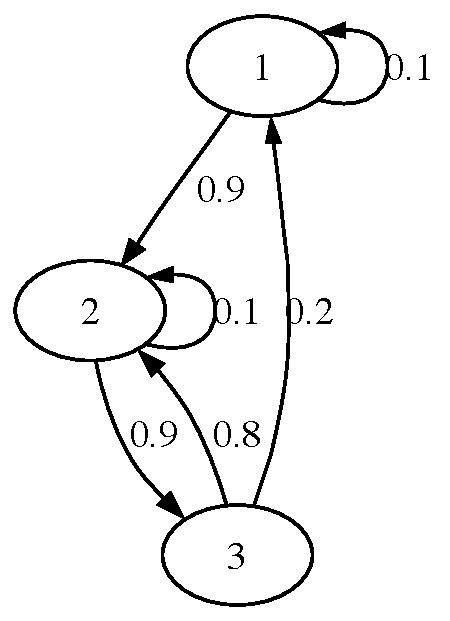
\includegraphics[scale=0.5]{smallmarkov}
  \end{minipage}
  \begin{minipage}{0.4\textwidth}
   $\displaystyle P = \left [ 
      \begin{array}{ccc} 
        0.1 & 0.9 & 0 \\ 
        0 & 0.1 & 0.9 \\ 
        0.2 & 0.8 & 0 
      \end{array} \right ]$
  \end{minipage}
  \caption{Markov process represented by a transition matrix and a graph}
  \label{fig:markovgraph}
\end{figure}

The state transition probabilities sufficiently describe the time
dependence of the process, but the initial state can not be determined
using the transition probabilities alone.  The probability of the
process starting out in a given state $i$ is denoted $\pi_i, i \in S$,
and the vector of initial state probabilities is called
$\boldsymbol{\pi}$. It can be seen that a discrete time Markov process
is completely described by its state space $S$, its state transition matrix
$P$ and its initial state probability vector $\boldsymbol{\pi}$.  If
$S$ is countable and has $N$ elements, $N^2 + N$ probabilities have to
be known to fully characterise the process.  For convenience, the
model is written $\lambda = (P, \boldsymbol{\pi})$.

\subsection{Hidden Markov Models} 
It is not always possible to observe the state (in the state space
$S$) of a Markov process directly. It may, however, be possible to
make observations from an observation space $O$ related to the state
of the process. If the probability of making a particular observation
is only related to the current state of the process, the process may
be described by a hidden Markov model (HMM). What is ``hidden'' in
this case are the true values of the Markov process states.

Figure~\ref{fig:hiddenmarkov} shows the situation graphically. If the
Markov process is in state 1, there are even odds that observation 2
or 3 will be made. In state 2, only observation 2 is made and state 3
is associated with observation 1 80\% of the time and observation 2
20\% of the time.

\begin{figure}[htbp]
  \centering
  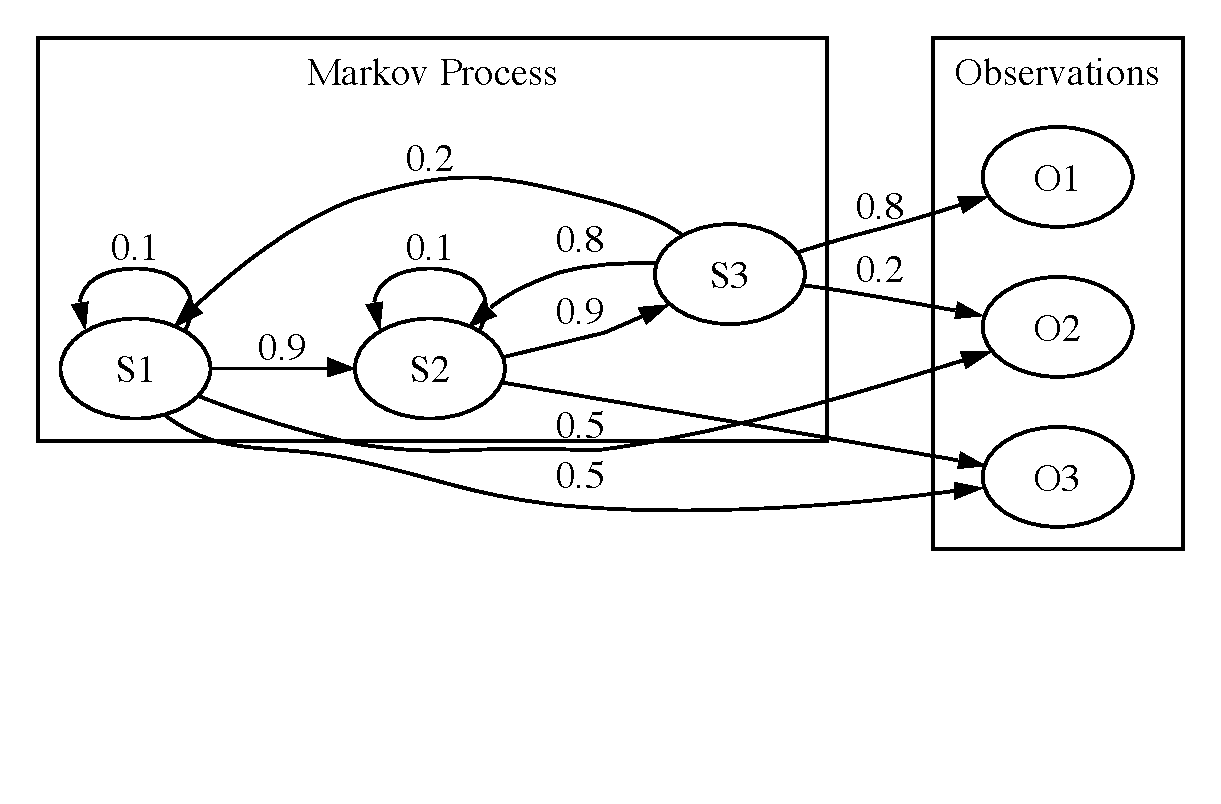
\includegraphics[scale=0.5,clip,trim=0 4cm 0 0]{smallhiddenmarkov}
  \caption{Graphical representation of a finite hidden Markov model}
  \label{fig:hiddenmarkov}
\end{figure}

The probabilities associated with a observation $k$ being made when
the process is in state $i$ may be written $b_{ik}$ and can be
arranged into an observation probability matrix $B$ in a similar
fashion as was previously done for $P$. One difference is that, while
$P$ was an $N \times N$ square matrix, $B$ will have $N$ rows
associated with the $N$ states of the Markov process and $M$ columns
associated with the observation space. An HMM as described here can
therefore be characterised by the same $N^2+N$ probabilities describing
the Markov process in addition to $MN$ observation probabilities.  The
model description can be abbreviated to $\lambda = (P, B, \boldsymbol{\pi})$.

There are three main problems associated with HMMs \citep{gamerman_markov_2006}:
\begin{itemize}
\item What is the probability of generating a specific output sequence
  from a particular model?
\item What is the most likely sequence of states that would lead to a
  particular output sequence?
\item How do we identify the model that corresponds to a given output
  sequence?
\end{itemize}

\subsection{Continuous-time Markov Processes}
The description of discrete-time Markov processes assumed that the
transition time was known or unimportant and one could imagine
simulating the process by picking a state $i$ and moving to the next
state with probability $p_{ij}$.  One shortcoming of such a
description is that there is no information about the amount of time a
process remains in a particular state before moving to the next (or
possibly same) state.  

Continuous-time Markov processes encode the transition probabilities as
transition rates $q_{ij}$ (forming a $Q$ matrix as $p_{ij}$ formed a
$P$ matrix), such that
\begin{equation}
  \label{eq:contmarkov}
  \Pr(X(t+\Delta t) = j | X(t) = i) = 
  \begin{cases}
    1 - q_{ii}\Delta t + o(\Delta t) & \text{for } i = j \\
    q_{ij}\Delta t + o(\Delta t) & \text{otherwise}
  \end{cases}
\end{equation}

The idea is that, having changed to a particular state the probability of moving to the next one approaches one over time, but at different rates.


\subsubsection{Application}
As an example of the results obtainable using multi-objective
optimisation, the MOPSO-CD (Multi-Objective Particle Swarm
Optimisation with Crowding Distance) algorithm proposed by\cite{raquel_effective_2005}was used to fit a first-order response
prototype to input signals.  The algorithm is a modification of
Particle Swarm Optimisation that adds an archive of nondominated
solutions and uses a crowding distance measure to prevent many similar
Pareto optimal solutions from being retained in the archive.

A problem description based on a prototypical first order response was
used in this study. Figure~\ref{fig:definition} shows the prototype
function.
\begin{figure}[htbp]
  \centering
  \setlength{\unitlength}{1.8em}
  \begin{picture}(10,10) 
    \thicklines
    % axis
    \put(1,1){\vector(1,0){8}}
    
    \put(5,0){$t$}
    \put(1,1){\vector(0,1){8}}
    \put(0,7){$y_p$}
    % curve
    \qbezier(2,2)(4,8)(8,8)
    \put(2,2){\circle*{0.2}}
    \put(2,0){$t_{i-1}$}
    \put(0,2){$y_{i-1}$}

    \put(8,8){\circle*{0.2}} 
    \put(8,0){$t_i$}
    \put(0,8){$y_i$}

    \put(3,2){$\Delta t$}
    \put(3,1.8){\vector(-1,0){1}}
    \put(3,1.8){\vector(+1,0){2}}

    \put(6,1.7){$\Delta t_i$}
    \put(6,1.5){\vector(-1,0){4}}
    \put(6,1.5){\vector(+1,0){2}}
    
    \thinlines
    \put(2,2){\line(-1,0){1}}
    \put(2,2){\line(0,-1){1}}
    \put(8,8){\line(-1,0){7}}
    \put(8,8){\line(0,-1){7}}
    \put(5,7){\line(-1,0){4}}
    \put(5,7){\line(0,-1){6}}

  \end{picture}
  \caption{First order response prototype definition.  $\Delta t$ and
    $\Delta t_i$ are the times of the interpolation time and end point
    time relative to the prototype start.}
  \label{fig:definition}
\end{figure}

Our goal is to find a sequence of prototypes that fits the sequence of
events.  We wish to fit the entire data set, so the first and last
times are to coincide with the first and last times in the data set.
Therefore, given that we are fitting $N$ prototypes, we seek to find
$N-1$ transition times and $N$ parameter value sets.

A few key decisions ease optimisation.  Firstly, a linear term 
added to the exponential response ensures that the prototype
interpolates through the initial $(x_{i-1}, y_{i-1})$ and final
$(x_{i}, y_{i})$ points.  This does add any parameters to the
description.  The predicted value for the prototype at a given time
$t$ is shown in equation~\ref{eq:prototype}:
\begin{equation}
  \label{eq:prototype}
  y_p = y_{i-1} + y_i \left (1 - \underbrace{e^{\Delta
        t/\tau_i}}_{\textrm{exponential}} + \underbrace{\frac{\Delta
        t}{\Delta t_i}e^{\Delta t_i/\tau_i}}_{\textrm{linear}} \right)
\end{equation}

Secondly, the optimisation parameters were chosen to reduce coupling
in the problem parameters by using absolute times for each starting
point and constraining these times to be sequential rather than time
differences constrained to be positive.  This reduced the effect of
any one starting point on the error produced by the remaining fit
functions.

\subsubsection{Objective functions}
Two objectives were defined: the RMS error of the fit over all the
prototypes and the ``complexity'' of the fit, which was calculated as
\begin{equation}
  c = \sum_i^{N} \frac{1}{\tau_i}.
\end{equation}

This complexity measure works due to the addition of the linear
correction term, which dominates for large $\tau$, meaning that as
$\tau$ increases, one sees more of the linear behaviour and less of
the exponential.  Therefore, larger $c$ corresponds to greater
curvature of the fitting prototypes.

\subsubsection{Prototype to event mapping}
Each sequence of prototypes identified was mapped back to a sequence
of event types by using the following heuristics:
\begin{itemize}
\item If the difference between the start and end values is less
  than a cut-off value $\epsilon_c$, the prototype is taken to
  represent a constant event.
\item If the time constant is larger than a cut-off time constant
  $\tau_c$, it is taken as a ramp.
\item If neither of these holds, the prototype is a first order response.
\end{itemize}

The values of $\epsilon_c$ and $\tau_c$ are problem-dependant and
should be chosen to represent an insignificant change in $y$ and a
large time constant (in the chosen time units) respectively.


\subsubsection{Results}
To illustrate the type of result that is obtained using the technique,
we show the results on a a signal consisting of 6 events, attempting
to fit 4 events.  Figure~\ref{fig:front_evolution} shows the evolution
of the Pareto front in terms of fit complexity and RMS error for
different numbers of iterations.

\begin{figure}[htbp]
  \centering
  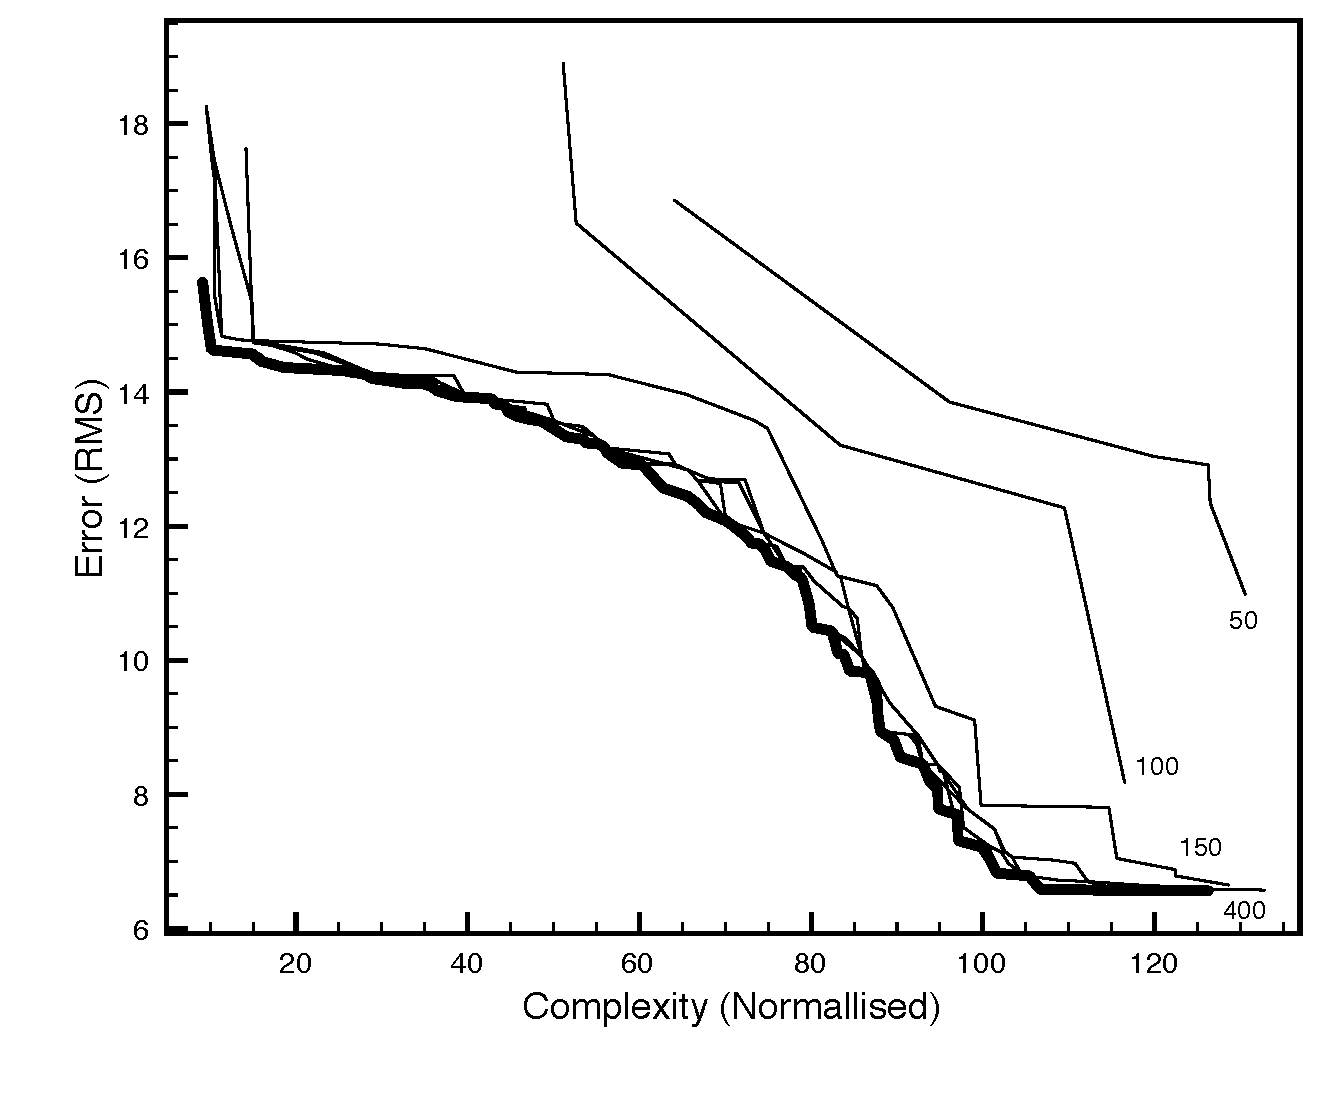
\includegraphics[width=0.7\textwidth]{front_evolution}
  \caption{Evolution of Pareto Front for 6 events being fit by 4 events.}
  \label{fig:front_evolution}
\end{figure}

It should be noted that, although the front seems to be converging,
population based multi-objective optimisation algorithms can not
guarantee convergence with a finite archive.  This is due to the
pruning that must inevitably be done when the archive is full.
Figure~\ref{fig:front_evolution} does, however, show that the front has not
receded.

\subsection{Optimisation with variable numbers of events}
The optimisation methods discussed so far have a significant
disadvantage: it is not possible for them to choose the ``optimal''
number of segments as one of the design variables, as their design space
needs to have constant dimension. It is, however, possible to use
genetic algorithms (GAs) for this purpose, by using a crossover
operator allowing varying chromosome lengths.  One such operator is
the simple ``cut and splice'' operator, which chooses a crossover
point on the chromosome of each parent independently before exchanging
material.  The application of multi-objective GAs with varying
chromosome lengths may yield the first fully-automated optimisation
for fitting events, as it allows the number of events to be included
in the objective set.

Finding the Pareto-optimal set of fits in this way will enable much
richer analysis of time series.

\section{Estimating state transition probabilities}
The most direct method of estimating the state transition
probabilities of a Markov process is to count the number of
transitions in an input signal.  This strategy has some problems:
\begin{enumerate}
\item Certain transitions may not occur in the input signal, so that
  these transitions will never be simulated by the identified model
\item Segmentation of the input signal may bias the event types or
  transitions -- if a certain event is more often fit by the
  segmentation algorithm, that event will be over-represented in the
  transition matrix.
\end{enumerate}

If transitions between some events are very rare, it may be advisable
to introduce a small artificial probability into the matrix to ensure
that the event has a chance of  getting generated during the
simulation.  This is especially true if the repercussions of a certain
event combination are significant.  

Segmentation bias can be combated by generating a large unbiased test
set and testing the segmentation algorithm on it.  If a segmentation
bias is detected, the transition probabilities can be modified to take
these into account.

% \section{Simulation}
% At the heart of any computer-based stochastic simulation is the
% generation of pseudo-random numbers.  It is customary to have a good
% source of uniformly distributed random numbers and to derive other
% distributions from them using either transformation or rejection
% methods.

% Most modern computer programming languages have at least this source
% of randomness, and some may include sources for normally distributed
% random values.  Commonly encountered transform methods can generate
% normally distributed, Poisson and logarithmically distributed vales
% from uniformly distributed values.~\citep{ripley_stochastic_2006}

% Direct simulation of Markov processes boils down to moving from state
% to state with the prescribed probabilities.  A simple way to choose
% values with specific probabilities is to use the cumulative sum of the
% probability vector associated with the current state.  When a 

\section{Conclusions}
Markov processes provide a simple yet powerful method for generating
realistic input sequences.  The theory in this chapter should be
enough for the interested reader to get started in this fascinating
field and should enable simulation of a system with little additional
reading required.  The techniques for segmenting input signals and
identifying model parameters are applicable to a broad range of fields
and includes novel work on the employment of multi-objective
optimisation to signal segmentation and estimation.

The most interesting future work suggested by this research is the use
of variable-length multi-objective GAs to segment signals.


% Local Variables:
% TeX-master: "thesis"
% End:


\chapter{Software}
\label{chap:software}
\begin{overview}
  Even though solving a set of model equations by hand can also be seen as simulation~\citehere, modern simulation will almost certainly involve using computers and computer programs.
  The act of simulation (ie the actual solution of the modelling equations) is also not the only process which benefits by using computers.
  Simulation generates data, which need to be stored and analysed in some way.
  The model descriptions themselves need to be encoded and stored.  
  This chapter reviews simulation-related software in this larger context, discussing current technology for developing models, solving the model
  equations and storing the resulting data.
  More attention is given to open-source software than to commercial software, as the framework is to use open source tools.
  The choices that have  been made for the modelling framework are interspersed in this discussion.
\end{overview}

\section{Model representations}

\subsection{Language based}

ProMOT \url{http://www.mpi-magdeburg.mpg.de/projects/promot}

Modelica

\subsection{XML based}

SBML \url{http://sbml.org/}


\subsection{Binary}


\section{Workflow}
NSF 

\subsection{What should workflow do?}

\subsection{Workflow tools}
% See:
% ~/Downloads/Documents/workflow
% ~/Downloads/Documents/workflow/scientific

\url{http://wiki.cogkit.org/index.php/Scientific_Workflow_Survey}

wftk \url{http://www.vivtek.com/wftk/perl_tutorial/08-workflow.html}
Perl-based single developer toolkit.  Good documentation about what
should go into a workflow tool.

Look into:
\begin{itemize}
\item \url{http://pegasus.isi.edu/wms}
\item \url{http://cppwfms.sourceforge.net}
\item \url{http://messagelab.monash.edu.au/Nimrod}
\end{itemize}

\subsection{Workflow specification languages}

\subsubsection{YAML}
\url{http://www.yawlfoundation.org} Very generic - examples are all
business workflows, has support for organisation model.  

\subsubsection{BPML}
Also for business.

\section{Concurrency}
\subsection{Local parallalism}

\section{Property packages}


\section{Simulators}
\subsection{Circuit simulators}
Spice
Gnu cap \url{http://www.gnu.org/software/gnucap/}
\subsection{Proprietary chemical systems}

\subsection{Modelica}
The Modelica project was spearheaded by \xxx, who started research on
modelling languages during his PhD studies in \xxx.  ``Modelica is a modern, strongly typed, declarative, and object-oriented language for modeling and simulation of complex systems.'' (\url{http://citeseerx.ist.psu.edu/viewdoc/summary?doi=10.1.1.139.7209})

\subsection{Stochastic simulation}
\subsubsection{Gnu MCsim}
From the MCSim users manual (\url{http://www.gnu.org/software/mcsim/mcsim.html}):
\begin{quote}
MCSim is a general purpose modeling and simulation program which can performs "standard" or "Markov chain" Monte Carlo simulations.
It allows you to specify a set of linear or nonlinear algebraic equations or ordinary differential equations. 
They are solved numerically using parameter values you choose or parameter values sampled from statistical distributions. 
Simulation outputs can be compared to experimental data for Bayesian parameter estimation (model calibration).
\end{quote}

\subsection{Proprietary simulators}
\subsubsection{gPROMS}

\subsubsection{SPEEDUP}

\subsubsection{HYSIS}

\subsubsection{CHEMCAD}

\subsection{Zero cost}
\subsubsection{Model.la}
% Model.la_Jerry_Bieszczad_phd.pdf
By a student of Stephanopolous. \url{http://web.mit.edu/modella/}

\subsubsection{COCO}
COCO simulator - Based on the Cape Open standard.  \url{http://cocosimulator.org/}

\subsection{Open source}

\subsubsection{ASCEND}
ASCEND from Carnegie Mellon university.  From the ASCEND website: \url{http://ascend.cheme.cmu.edu/}
\begin{quote}
  ASCEND is a system for solving systems of equations, aimed at engineers and scientists. It allows you to build up complex models as as systems constructed from simpler sub-models. Using ASCEND it is simple to play around with your model, examine its behaviour, and work out how it can best be solved. You can easily change which variables are fixed and which are to be solved, and you can examine the way in which the model is being solved.
\end{quote}
\subsubsection{EMSO}
%TODO: Check out EML the EMSO model library
EMSO process simulator from ALSOC (\url{http://www.enq.ufrgs.br/trac/alsoc}).

From the EMSO website:
\begin{quote}
EMSO is the acronym for Environment for Modeling, Simulation, and Optimization. 
EMSO is a graphical environment where the user can model complex processes simply selecting and connecting the equipment models. 

The main features of EMSO follows: 

\begin{itemize}
\item Entirely written in C++
\item A fairly portable code, currently
  available for Windows and Linux but can be compiled for other
  platforms if desired
\item It is an Equation-Oriented simulator The unique
  Equation-Oriented simulator with units-of-measurement checking for
  the equations
\item A large set of built-in functions
\item Models are written
  in a modeling language, the user does not need to be a programmer

\item Models are converted to system of equations in memory, no
  compilation or linking is needed
\item An open library of models, called
  EML
\item Built-in code for symbolic differentiation which enables the
  system to solve high-index problems
\item Built-in code for automatic
  differentiation which makes the system very efficient
\item Can make use
  of machine optimize BLAS routines
\item Currently support: 
  \begin{itemize}
  \item static simulation
  \item dynamic simulation
  \item static optimization
  \item parameter estimation of static models
  \item parameter estimation of
    dynamic models
  \end{itemize}
\item A
  graphical user interface which can be used to model development,
  simulation execution, and results visualizing
\item A system of PlugIns where the user can embed code written in C,
  C++ or FORTRAN into the models A very modular system - all solvers
  are DLL's and the user can even write their own NewSolver Models
\end{itemize}
\end{quote}

\subsubsection{DWSIM}
\label{sec:dwsim}

From the DWSIM website: \url{http://dwsim.inforside.com.br/}
\begin{quote}
DWSIM is a Chemical Process Simulator for Windows. Built on the Microsoft .NET 2.0 Platform and featuring a rich Graphical User Interface (GUI), DWSIM allows chemical engineering students and chemical engineers to better understand the behavior of their chemical systems by using rigorous thermodynamic and unit operations' models with no cost at all. Even better, they can see how the calculations are actually being done - DWSIM is open source, that is, its code is available to anyone who wishes to discover the "magic" behind it or just do some code browsing. 
\end{quote}

\subsubsection{OPSIM}
\label{sec:opsim}
Windows-only.  \url{http://sourceforge.net/projects/opsim/}

\section{Programming languages}
\citep{chaves.nehrbass.ea2006octave}

\section{Data formats}
\subsection{Time-series data}
Input and output time-series

\subsection{Properties}
See CAPE-Open

\subsection{Object data}
Data requirements of each unit/storage

\section{Data technologies}
\subsection{Relational databases}
\subsection{HDF5}

\section{CAPE-OPEN}
The CO-lan describes CAPE-OPEN as follows:
\begin{quote}
CAPE-OPEN standards are the uniform standards for interfacing process modelling software components developed specifically for the design and operation of chemical processes. 
They are based on universally recognized software technologies such as COM and CORBA. 
CAPE-OPEN standards are open, multiplatform, uniform and available free of charge. 
They are described in a formal documentation set.
\end{quote}

The documentation set comprises the following items:
\subsection{Thermodynamics and Physical Properties Interface Specification}

\subsection{Unit Operations Interface Specification}

\subsection{Chemical Reactions Interface Specification}

\subsection{Methods \& Tools Integrated Guidelines}

\subsection{Optimisation Interface Specification}

\subsection{Parameter Estimation and Data Reconciliation Interface Spec}
This document defines the interfaces required to do parameter estimation and data reconciliation.  
The parameter estimation problem is to find the parameters that correspond with the best match between the model and the data, while the data reconciliation problem is to find data that does not correspond to the model.  
Both of these activities require a model of the system or the ability to run the model and data from the system.  

\subsection{Partial Differential Algebraic Equations Interface Specification}

\subsection{Petroleum Fractions Interface Specification}

\subsection{Physical Properties Data Bases Interface Specification}

\subsection{Planning and Scheduling Interface Specification}

\subsection{Simulation Context COSE Interface}


\subsection{Identification Common Interface}
\subsection{Parameter Common Interface}
\subsection{Collection Common Interface}
\subsection{Error Common Interface}
\subsection{Persistence Common Interface}
\subsection{Utilities Common Interface}

\section{Complex event processing}
% TODO: Flesh out
Identification of multiple events in a stream of events as a single event is being done under the name ``Complex event processing'' \url{http://en.wikipedia.org/wiki/Complex_event_processing}.  
This is mostly done in the field of business intelligence.  

% Local Variables:
% TeX-master: "thesis"
% End:


\chapter{Test problems}
\begin{overview}
To verify that the system is working correctly, it is important to define tests.
This chapter describes the test data and systems that will be used to test the simulation system.
Some of these systems are widely used, while some of them are sourced from industry or synthetic.
\end{overview}

\section{Statistical analysis}
A library of signals exhibiting each of the statistical properties discussen in section~\ref{}

\section{Segmentation datasets}
\subsection{On-line data from distillation unit}
Originally, the LPG section was desinged to take a C2, C3 and C4 parrafinic feed and separate the components to final products. 
The C2 material was separated in VL103 and sent to the HP flare under pressure control. 
VL104 separated the C3 and C4 components.
 
Since then, the feed composition changed with C2's no longer present under normal operating conditions. 
However, there are occational C2 breakthrough in the feed.
 
Cuurently, the lack of C2's makes pressure control very difficult in Vl103. 
This causes the column profile to rise and fall, wich causes alot of instability in the system Set 1 and 2 of the data contain the most recent control changes on the plant. 
T1057 used to cascade to the steam flow. 
However, dynamic simulations suggested that the reflux flow could be used to control the steam flow. 
As the column moves to the top, the reflux flow will increase and this will cause a slow cut in steam and vice versa.
 
Set 3 contains the old configuartion where the temperature in the bottom was used to control the steam flow rate.
%TODO: Get data Petri supplied from Sasol and auto-segment

\begin{figure}[htp]
\begin{center}
  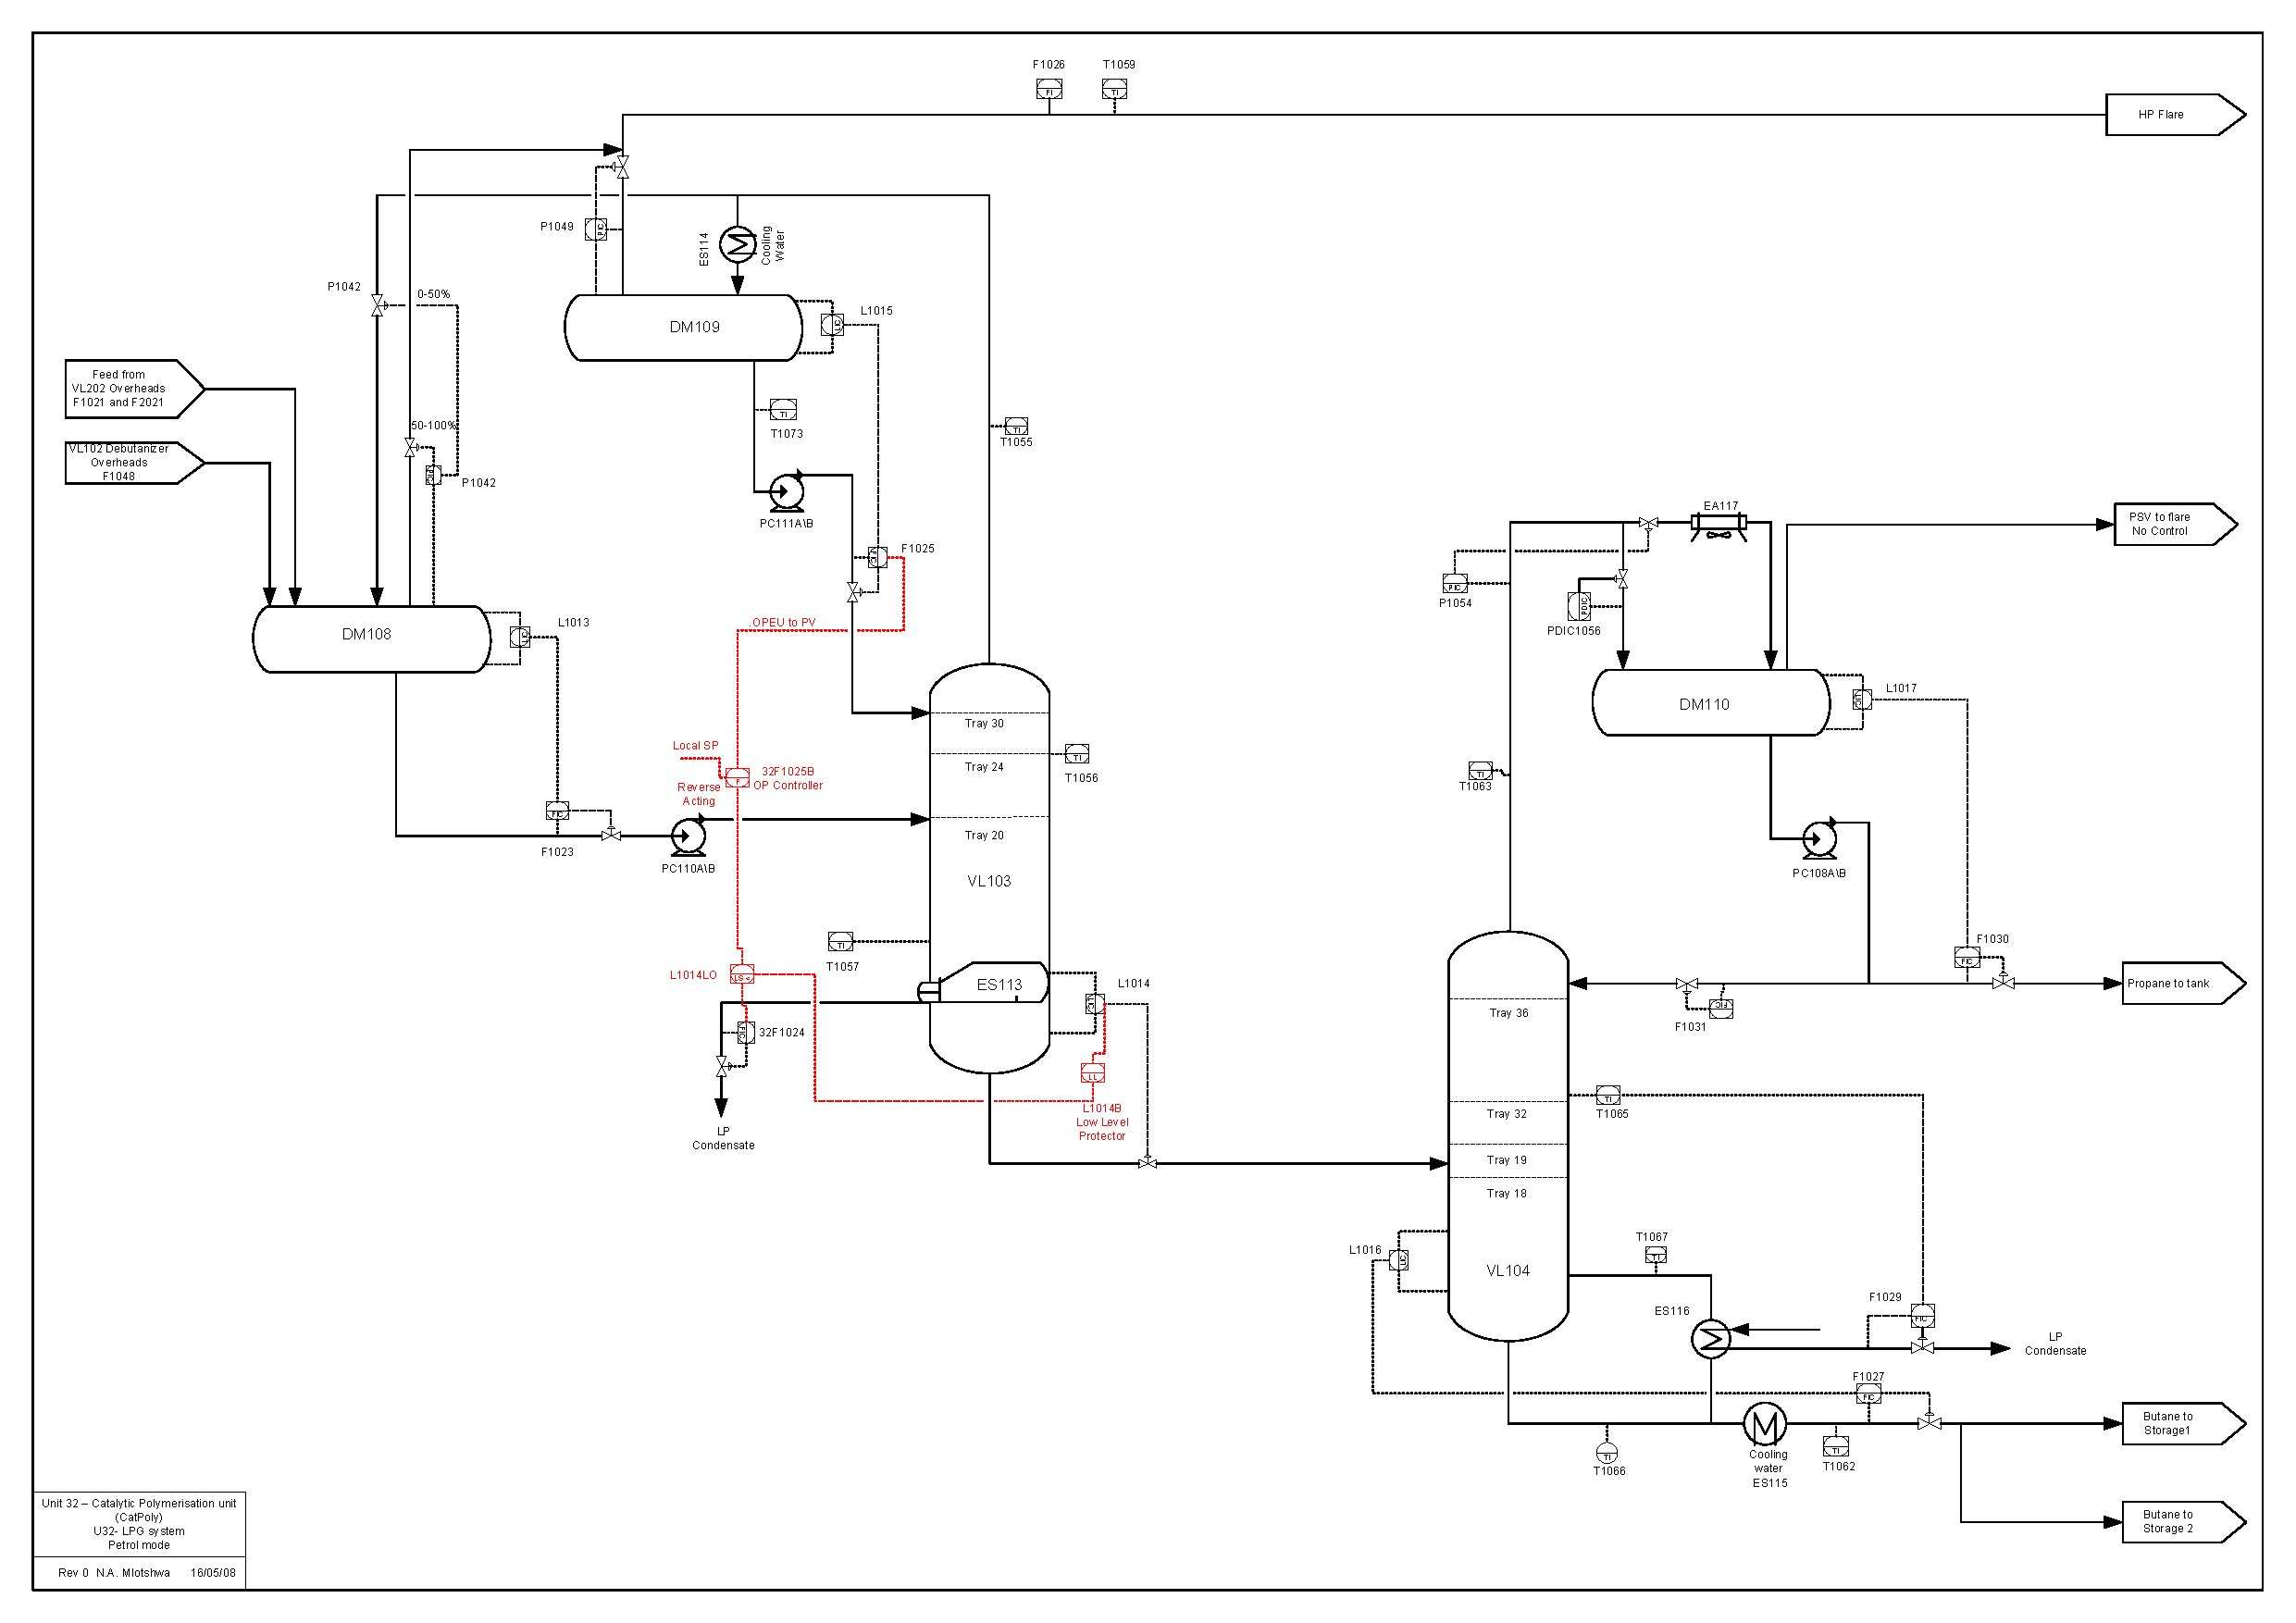
\includegraphics[width=\textwidth]{LPG_process}
  \caption[LPG process]{Industrial LPG process}
  \label{fig:lpgprocess}
\end{center}
\end{figure}

\section{Systems}
\subsection{Single tank}

\subsection{Two coupled tanks}
Allowing flow reversal

\subsection{Flash drum}

\subsection{Distillation column}

\subsection{Reactor}

\subsection{Reactor with flash drum and recycle}

\subsection{Tennessee Eastman challenge problem}
In 1993, \citet{downs.vogel1993plant-wide} proposed the Tennessee Eastman plant-wide Industrial control problem as a test for new control algorithms. 
The core of the process is a reactor with a separation and recycle arrangement.  
The flowsheet is shown in Figure~\ref{fig:teprocess}.
\begin{figure}[htbp]
  \centering
  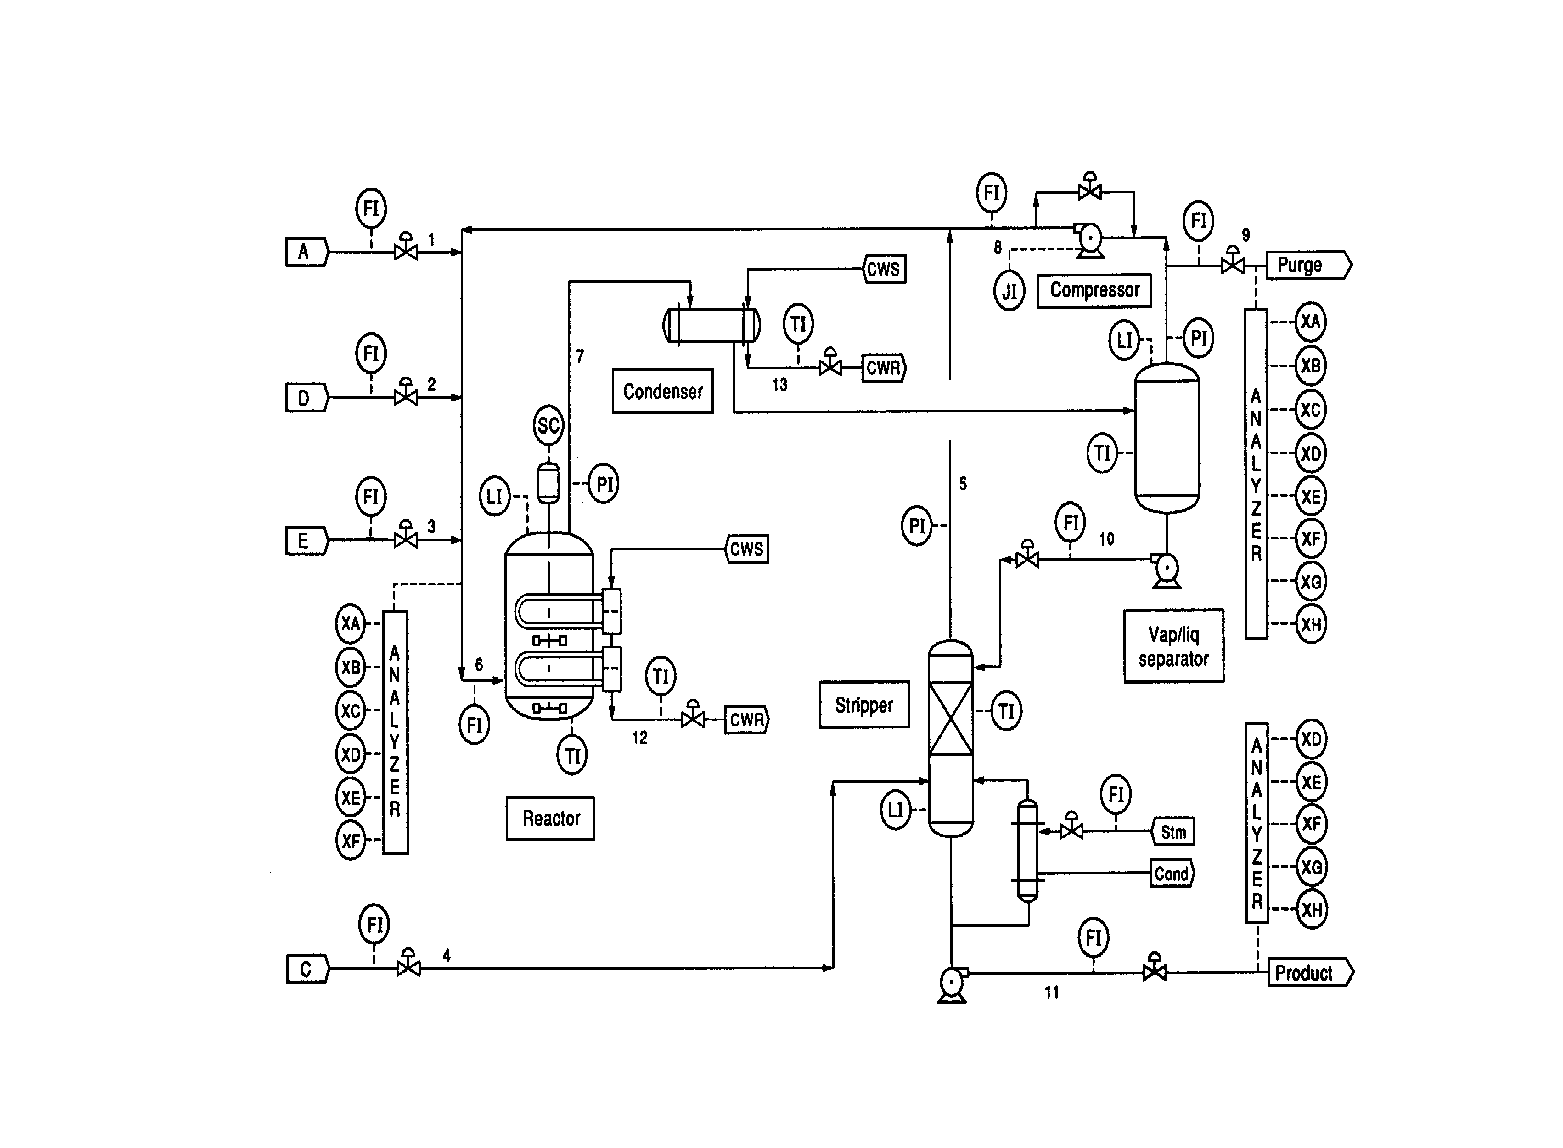
\includegraphics[width=\textwidth]{teflowsheet}
  \caption{Flowsheet for the Tennessee Eastman process~\citep{downs.vogel1993plant-wide}}
  % TODO: Redraw TE flowsheet properly.
  \label{fig:teprocess}
\end{figure}

Four reactions featuring eight compounds (A through H) take place in the reactor:
\begin{eqnarray}
A(g) + C(g) + D(g) & \rightarrow & G(l) \\
A(g) + C(g) + E(g) & \rightarrow & H(l) \\
A(g) + E(g)        & \rightarrow & F(l) \\
3D(g)              & \rightarrow & 2F(l) 
\label{eq:te-reaction}
\end{eqnarray}

G and H are the first and second products, while F is a byproduct.

% Local Variables:
% TeX-master: "thesis"
% End:


\part{Design and implementation}
\chapter{Background}\label{chap:background}
\begin{overview}
\end{overview}

% Local Variables:
% TeX-master: "thesis"
% End:

\chapter{Implementation}\label{chap:implementation}
\begin{overview}

\end{overview}

\section{Segmentation}\label{sec:imp:segmentation}
\subsection{The Segmentation module}
The techniques described in section \ref{chap:lit:segmentation} were all implemented in a Python module called \modulename{Python}{segmentation}.

\subsection{Multi-objective fitting}
% TODO: Replace the reference to raquel with a cross-reference to the optimization chapter
As an example of the results obtainable using multi-objective optimisation, the MOPSO-CD algorithm discussed in section~\ref{sec:mopso} was used to fit a first-order response prototype to input signals.

A problem description based on a prototypical first order response was used in this study. Figure~\ref{fig:definition} shows the prototype function.
\begin{figure}[htbp]
  \centering
  \setlength{\unitlength}{1.8em}
  \begin{picture}(10,10) 
    \thicklines
    % axis
    \put(1,1){\vector(1,0){8}}
    
    \put(5,0){$t$}
    \put(1,1){\vector(0,1){8}}
    \put(0,7){$y_p$}
    % curve
    \qbezier(2,2)(4,8)(8,8)
    \put(2,2){\circle*{0.2}}
    \put(2,0){$t_{i-1}$}
    \put(0,2){$y_{i-1}$}

    \put(8,8){\circle*{0.2}} 
    \put(8,0){$t_i$}
    \put(0,8){$y_i$}

    \put(3,2){$\Delta t$}
    \put(3,1.8){\vector(-1,0){1}}
    \put(3,1.8){\vector(+1,0){2}}

    \put(6,1.7){$\Delta t_i$}
    \put(6,1.5){\vector(-1,0){4}}
    \put(6,1.5){\vector(+1,0){2}}
    
    \thinlines
    \put(2,2){\line(-1,0){1}}
    \put(2,2){\line(0,-1){1}}
    \put(8,8){\line(-1,0){7}}
    \put(8,8){\line(0,-1){7}}
    \put(5,7){\line(-1,0){4}}
    \put(5,7){\line(0,-1){6}}

  \end{picture}
  \caption{First order response prototype definition.  $\Delta t$ and $\Delta t_i$ are the times of the interpolation time and end point time relative to the prototype start.}
  \label{fig:definition}
\end{figure}

Our goal is to find a sequence of prototypes that fits the sequence of events.  
We wish to fit the entire data set, so the first and last times are to coincide with the first and last times in the data set.
Therefore, given that we are fitting $N$ prototypes, we seek to find $N-1$ transition times and $N$ parameter value sets.

A few key decisions ease optimisation.  
Firstly, a linear term  added to the exponential response ensures that the prototype interpolates through the initial $(x_{i-1}, y_{i-1})$ and final $(x_{i}, y_{i})$ points.  
This does add any parameters to the description.  
The predicted value for the prototype at a given time $t$ is shown in equation~\ref{eq:prototype}:
\begin{equation}
  \label{eq:prototype}
  y_p = y_{i-1} + y_i \left (1 - \underbrace{e^{\Delta
        t/\tau_i}}_{\textrm{exponential}} + \underbrace{\frac{\Delta
        t}{\Delta t_i}e^{\Delta t_i/\tau_i}}_{\textrm{linear}} \right)
\end{equation}

Secondly, the optimisation parameters were chosen to reduce coupling in the problem parameters by using absolute times for each starting point and constraining these times to be sequential rather than time differences constrained to be positive.  
This reduced the effect of any one starting point on the error produced by the remaining fit functions.

\subsection{Objective functions}
Two objectives were defined: the RMS error of the fit over all the prototypes and the ``complexity'' of the fit, which was calculated as 
\begin{equation}
  c = \sum_i^{N} \frac{1}{\tau_i}.
\end{equation}

This complexity measure works due to the addition of the linear correction term, which dominates for large $\tau$, meaning that as $\tau$ increases, one sees more of the linear behaviour and less of the exponential.  
Therefore, larger $c$ corresponds to greater curvature of the fitting prototypes.

\subsection{Prototype to event mapping}
Each sequence of prototypes identified was mapped back to a sequence of event types by using the following heuristics:
\begin{itemize}
\item If the difference between the start and end values is less   than a cut-off value $\epsilon_c$, the prototype is taken to   represent a constant event.
\item If the time constant is larger than a cut-off time constant   $\tau_c$, it is taken as a ramp. 
\item If neither of these holds, the prototype is a first order response.
\end{itemize}

The values of $\epsilon_c$ and $\tau_c$ are problem-dependant and should be chosen to represent an insignificant change in $y$ and a large time constant (in the chosen time units) respectively.

\section{Model library}
\subsection{Stream type}
A key element in the development of a Modelica chemical engineering simulation library is the encoding of the stream data in a stream type.  

%NOTE: Design only - replace by what was actually implemented - this probably
% needs to be in a separate file.

Intensive properties:
\begin{itemize}
  \item Pressure
  \item Temperature
\end{itemize}

Exensive properties:
\begin{itemize}
  \item Component mass flow rates (compositions come from flowrates)
\end{itemize}

To start building the simulation, the components have to be chosen and the initialiser has to be run.  
This creates the stream types that can be used in the rest of the unit operations.  
Simulation will fail if the component list is changed without re-running the initialiser.	

\subsection{Connector philiosophy}
%NOTE: This is rambling, but I'm getting my thoughts on paper
Blocks in Modelica are connected by connector types.  
The variables in the connectors can connect as ``flow-type'' variables or ``potential-type'' variables.  
The difference is in how the sign of equality is handled when the model is constructed.  
Flow-type variables are connected with a negative sign (so that flow out of one block is equal to the flow into another, but in the opposite direction), while potential-type variables are simply set equal to one another (this works well for things like pressure).

It was decided to bundle the extensive properties of the stream and the intensive properties of the stream seperately.

\section{CORBA support}
There are two popular patterns for the use of CAPE-OPEN when developing custom simulation codes.  
The first is to make use of the Unit Operation support to embed a unit operation into an existing flowsheeting package, which then handles the simulation calculations. 
The second is to use a stand-alone modelling environment, but to interface with various packages for information like thermodynamic properties, equilibrium and/reaction kinetics.  
It was decided to abstract the property and equilibrium calculations into a class (SimulationStream) which is specified as a connector type for the column components.  
The SimulationStream objects that are instantiated when the components are simulated communicate with a host using the ICapeThermoPropertyPackage methods CalcProp and CalcEquilibrium.  
The interfacing is done using CORBA.  
Mico CORBA was used on the client (Linux) machine, accessed using the support for external C routines in OpenModelica.  
On the host (Windows) machine, the Unisim CORBA Server was used to interface with Unisim.

Figure~\ref{fig:dataflow} shows the data flow conceptually.
\begin{figure}[htbp]
  \centering
  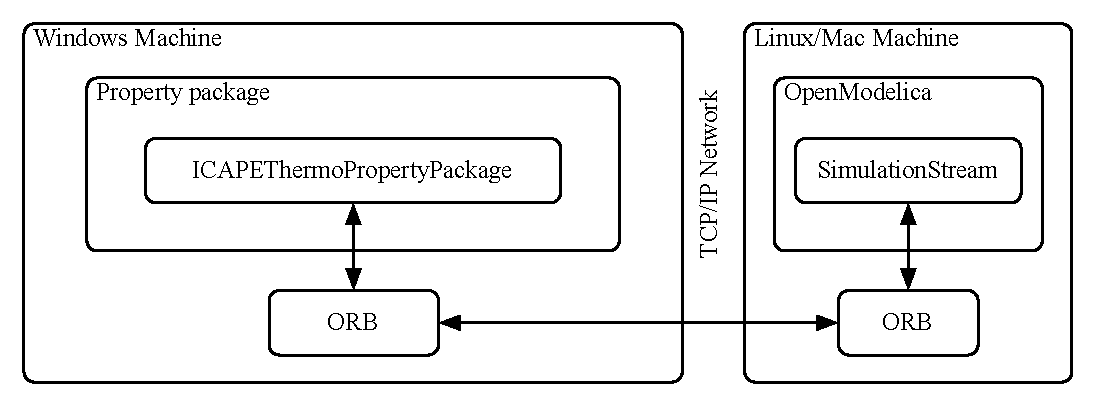
\includegraphics[width=0.9\textwidth]{dataflow}
  \caption{Simulation data flow for multiple computers}
  \label{fig:dataflow}
\end{figure}

It should be noted that, although this implementation has used CORBA due to the lack of support of COM on the Linux platform, CO-LaN supplies a COM-to-CORBA bridge as part of the CAPE-OPEN effort, so using CORBA is not a significant problem.

\section{Column model}
\label{sec:column-model} 
The distillation column modelled is a lab-scale glass distillation column fitted with a water-cooled total condenser and a steam thermosyphon boiler.  
It separates a mixture of ethanol and water.

The Modelica components developed for modelling the distillation column are shown schematically in Figure~\ref{fig:components}
\begin{figure}[htbp]
  \centering
  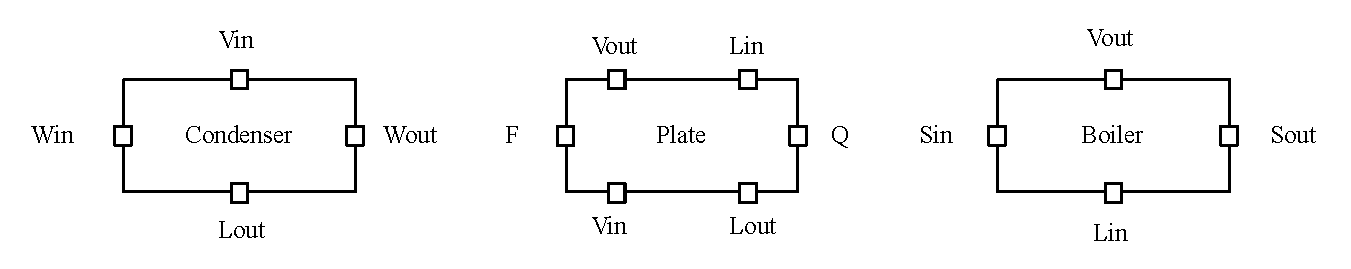
\includegraphics[width=\textwidth]{components}
  \caption{Distillation column components}
  \label{fig:components}
\end{figure}

A single generic plate model was developed that allows for a material and energy stream (both of which could be incoming or outgoing, labelled F and Q in the diagram) in addition to the normal vapour and liquid arrangement (two vapour streams and two liquid streams).  
This allows multiple feed columns to be modelled easily, even when the feeds are intermittend during the simulation.  
It also allows for energy losses or additions.  
The physical column that was modelled exhibits significant heat losses.

The plate model assumes negligible vapour dynamics, with per-component hold-up on the liquid side.  
The pressure drop between the input and output vapour streams is estimated using the height of liquid on the plate.  
The Wilson thermodynamic model was used as it accurately describes the ethanol-water equilibrium. 

The material streams these components are specified as SimulationStreams, allowing the material properties and equilibrium to be calculated by the external thermo host.


% Local Variables:
% TeX-master: "thesis"
% End:

\part{Results}
\chapter{Results}\label{chap:results}
\begin{overview}
  Results of the techniques whose implementation was discussed in the previous part are shown here.  
  The result of various event identification techniques are shown, followed by examples of models built using the Modelica package and the results of the simulation of these models.
\end{overview}

\section{Segmentation}\label{sec:res:segmentation}
%TODO: This was ripped from the ESCAPE-21 article.
Figure~\ref{fig:segmentationresults} shows some of the results the automated segmentation the sample input data.  
Note that this is a subset of all the fits done, for illustrative purposes.  

\begin{figure}[htbp]
  \centering
  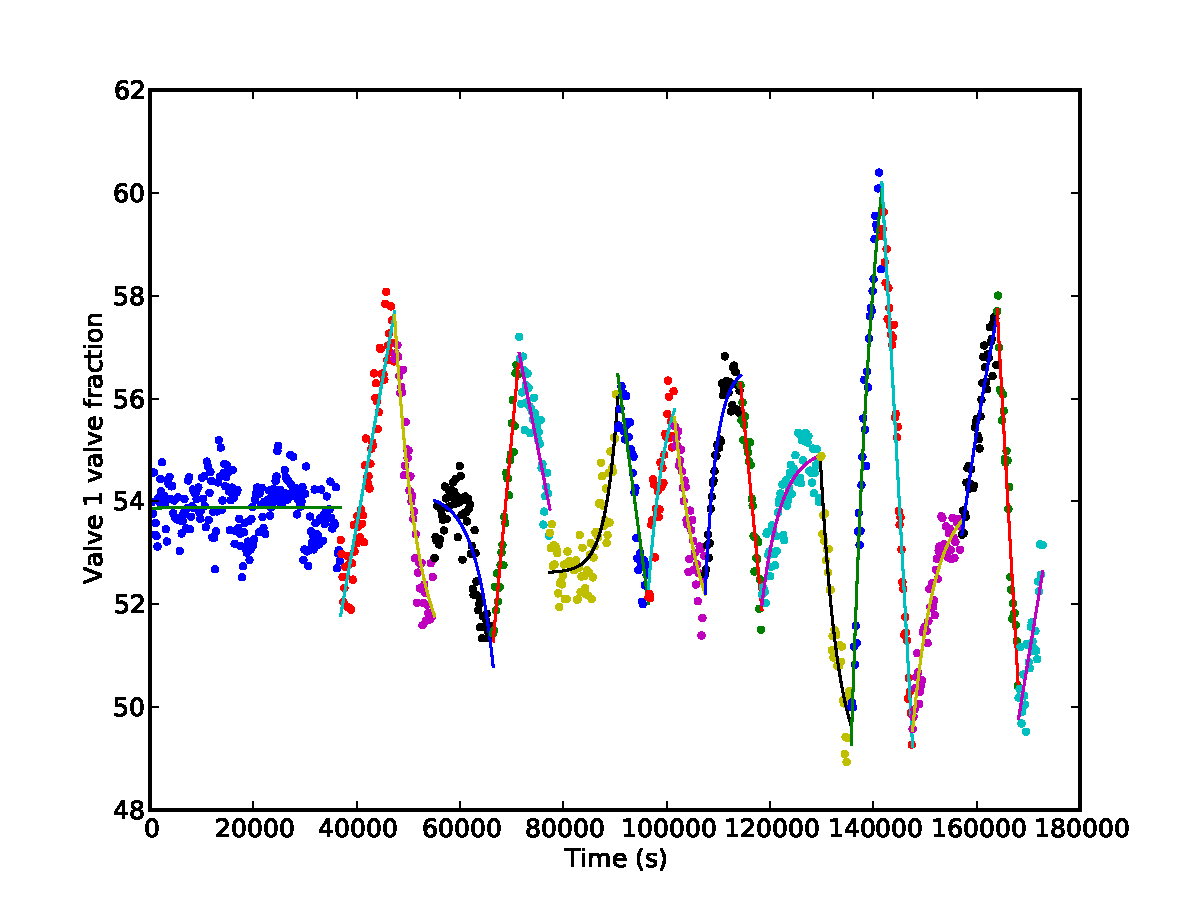
\includegraphics[width=0.7\textwidth]{segmentedsignal}
  
(a)

  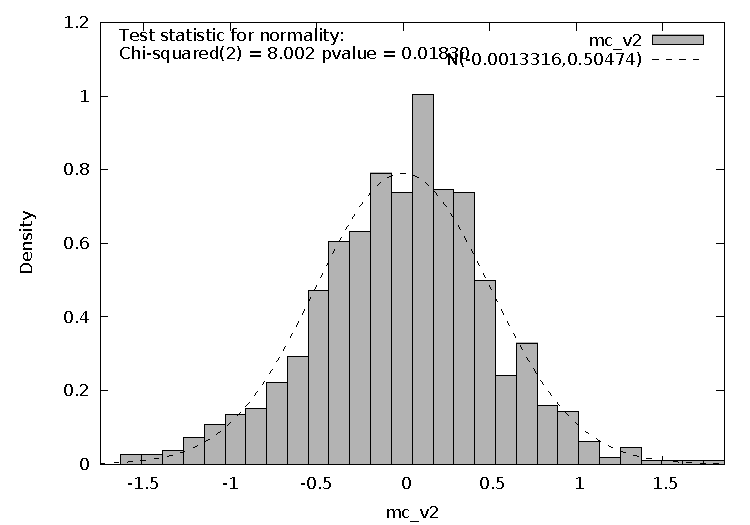
\includegraphics[width=0.44\textwidth]{teresidualnormality}

(b)

  \caption{Segmentation and signal generation results for TE valve input signal.  The residuals are normally distributed.}
  \label{fig:segmentationresults}
\end{figure}

The transitions were analysed for all the fits obtained.

The overall residuals were determined to have be approximately
normally distributed with a standard deviation near 0.5 as shown in Figure~\ref{fig:segmentationresults}.  
This increases the confidence in the segmentation as TE code makes use of normally distributed noise signals.

\subsection{Top-down}

\subsection{Bottom-up}

\subsection{Test signals}
To illustrate the type of result that is obtained using the technique, we show the results on a a signal consisting of 6 events, attempting to fit 4 events.  
Figure~\ref{fig:front_evolution} shows the evolution of the Pareto front in terms of fit complexity and RMS error for different numbers of iterations.

\begin{figure}[htbp]
  \centering
  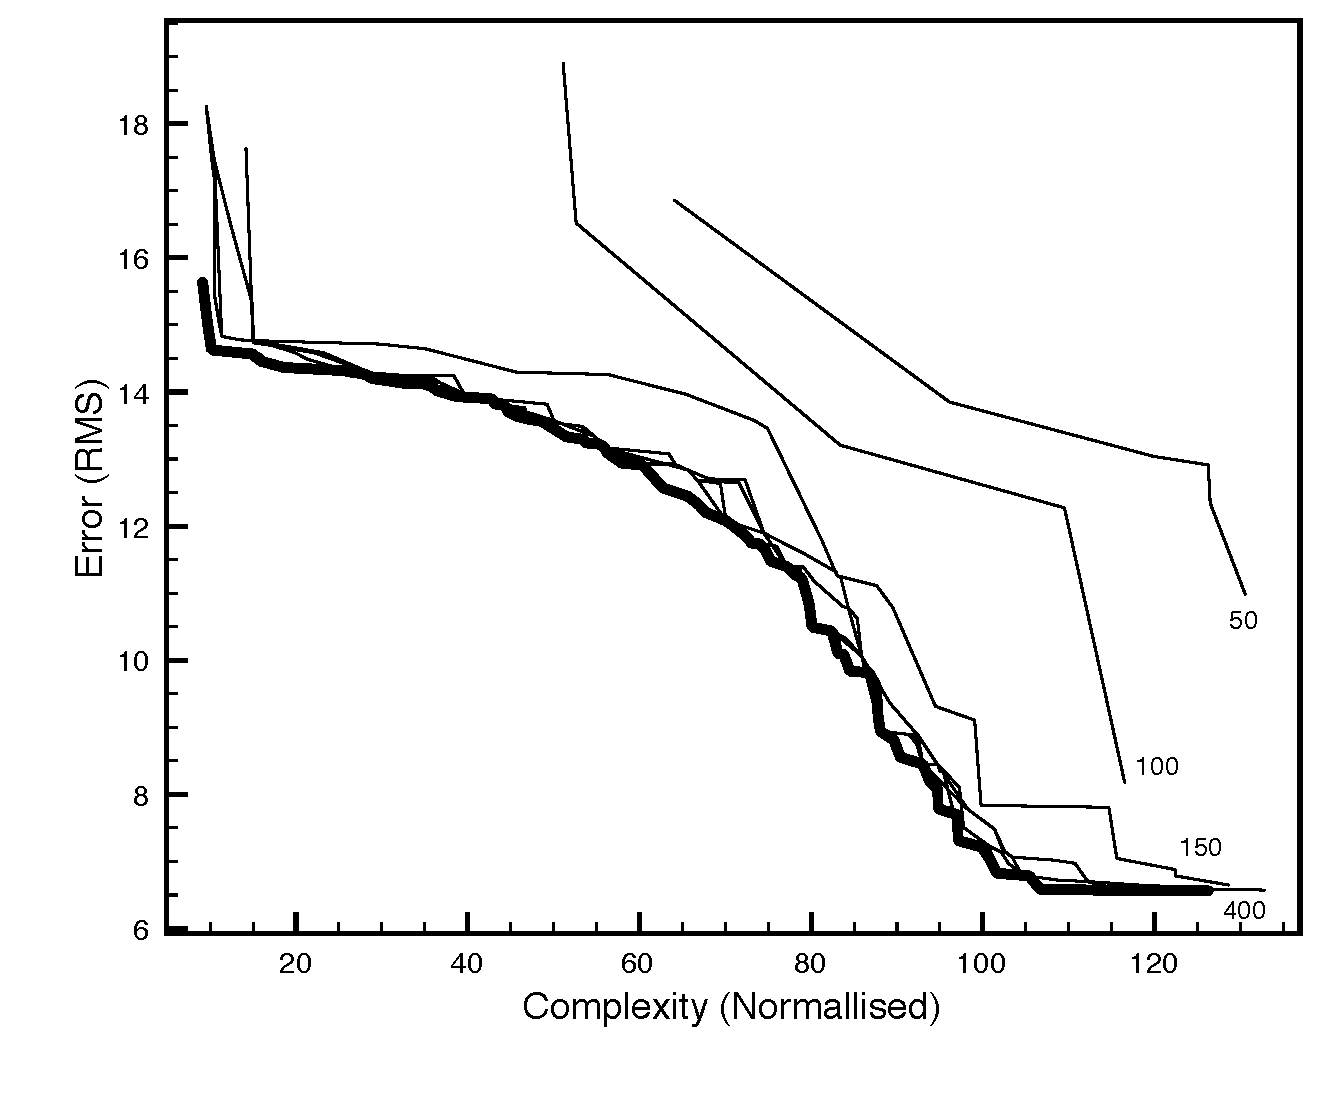
\includegraphics[width=0.7\textwidth]{front_evolution}
  \caption{Evolution of Pareto Front for 6 events being fit by 4 events.}
  \label{fig:front_evolution}
\end{figure}

It should be noted that, although the front seems to be converging, population based multi-objective optimisation algorithms can not guarantee convergence with a finite archive.  
This is due to the pruning that must inevitably be done when the archive is full.
Figure~\ref{fig:front_evolution} does, however, show that the front has not receded.

\subsection{Real-life signals}


\section{Models}

\section{Distillation column model}
\subsection{Simulation accuracy}
To verify the accuracy of the model, it was run simultaneously with the column.  
Figure~\ref{fig:comparison} shows the results of a sample run during which the feed flow rate was varied.  
The distillate drum level and the top plate (plate 1) temperature are shown to illustrate the behaviour of the column and the model.

\label{sec:results}
\begin{figure}[htbp]
  \centering
  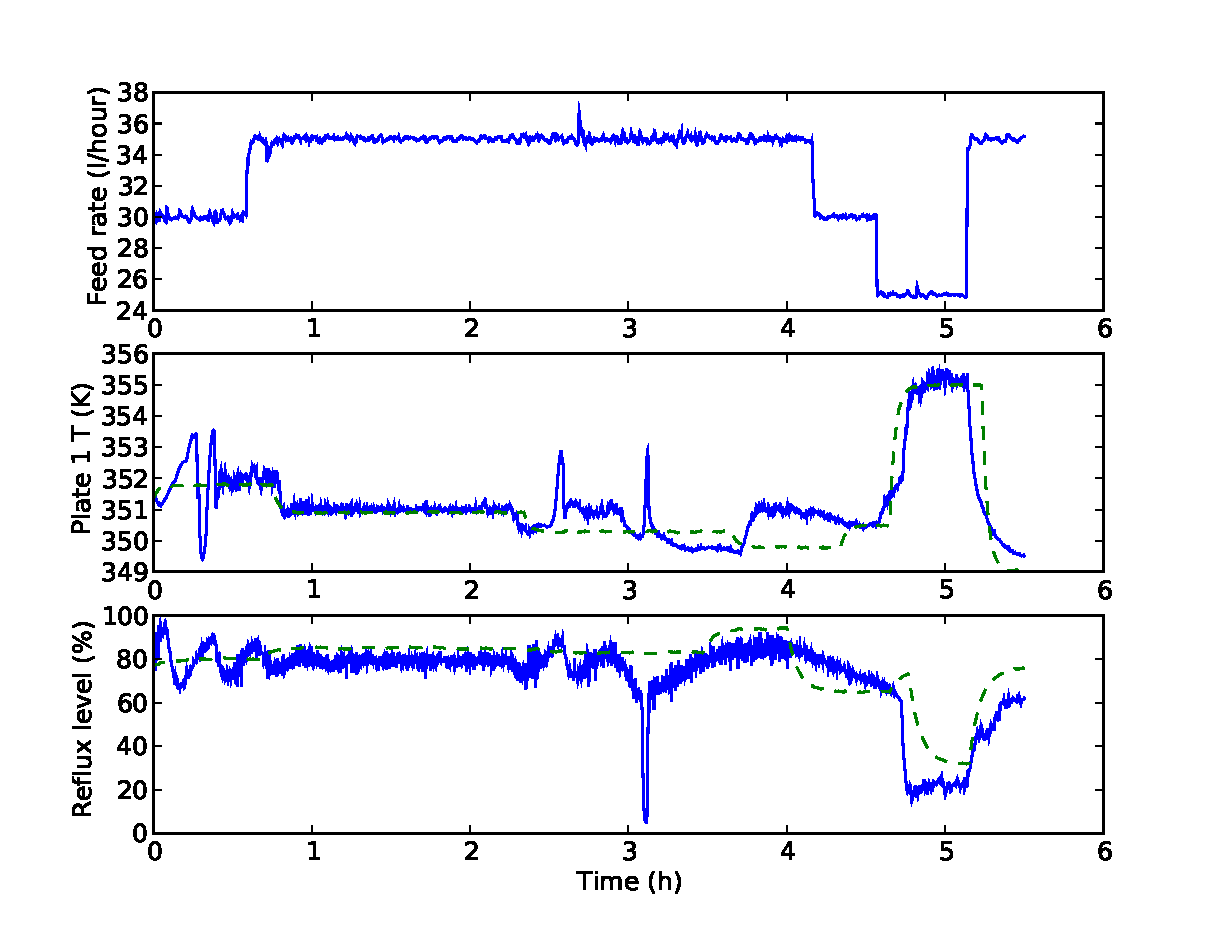
\includegraphics[width=0.9\textwidth]{comparison}
  \caption{Results of simulation compared to measurements. Solid lines are experimental results, dashed lines are model results.}
  \label{fig:comparison}
\end{figure}

It should be noted that the model does not accurately reflect the variation in the reflux drum, probably due to a mismatch between the controller parameters in the model and on the column.  
Further investigation into fitting model parameters should be done.  
However, the overall trends are similar, which is sufficient for this work.

\subsection{Performance profiling}
Real-time operation of the column model proved difficult, and in order to speed up the simulation, profiling of the components making up the simulation was done.  
It was found that the simulation itself could achieve several times real time when simple equilibrium from tables and constant material properties were used instead of the external thermodynamic package.  
As an example, simulating the run shown in Figure~\ref{fig:comparison} takes 30 minutes with simple thermodynamics and 4 hours using the external interface.  
Both the client and the host computers are Pentium 4 Machines with 1GiB of ram.

The high sampling rate of the data (which is sampled at 1 second intervals) may force the integration engine to generate a time point each second, accounting for some of the computational effort. 
However, due to the large difference in running the simulation with and without the external interface, it was surmised that the integration routines of OpenModelica (which uses the DASSL routine from netlib) are not entirely to blame.

In order to better understand the problem, the time spent in handling the network requests was logged.  
This is all the time spent blocked on the network request.  
The results are shown in Figure~\ref{fig:overhead}.
\begin{figure}[htbp]
  \centering
  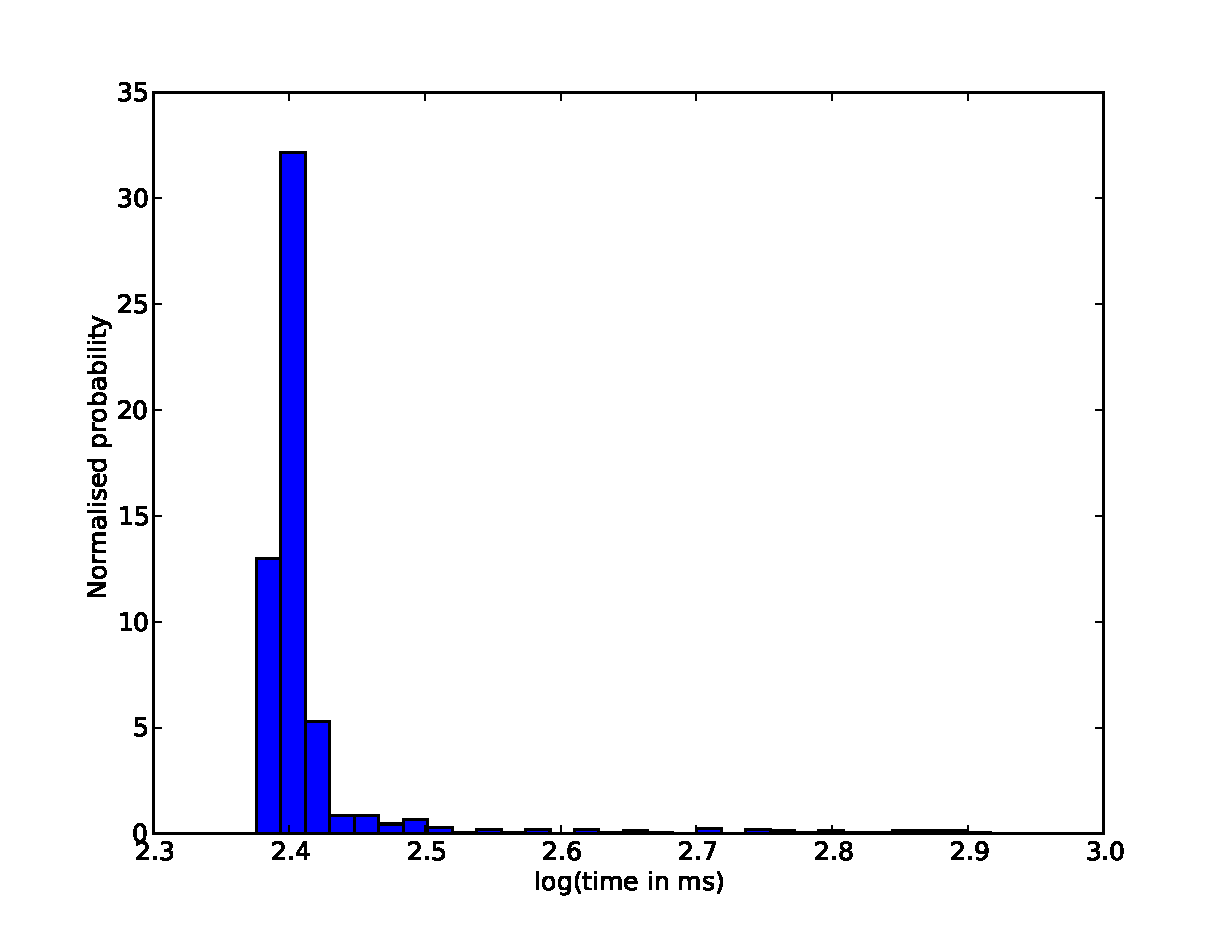
\includegraphics[width=0.6\textwidth]{nethist}
  \caption{Networking overhead for intensive simulation}
  \label{fig:overhead}
\end{figure}
Taking into account that a 30 minute simulation of about 20000 time steps translates to 90 ms per time step and 4 hours 720 ms per time step, it can be seen that the network-blocked part takes about 40\% of the simulation time in most cases, but can take the entire allocated time in some cases.  

The network overhead is therefore significant, even though not all of the performance issues can be attributed solely to the network layer. 
One other possibility that is being pursued is that the compilation of the model files when external routines are being used is not optimal.

A possible explanation for this is that there are SimulationStream instances which all communicate with the server.  
This adds a large overhead due to multiple connections being maintained and property traffic being transmitted simultaneously.  
Currently, work is underway to develop a data broker that will structure the requests to the ORB in a more efficient way.  
The possibility of caching some of the data is also being investigated.

Another explanation is that the external module does not supply derivative information when it is being evaluated, forcing the integration routines to resort to finite differences when estimating the derivatives of these units while solving the equations.  
Attempts are also being made to enable derivative information to be handled by the interface.

% Local Variables:
% TeX-master: "thesis"
% End:

\chapter{Conclusion and recommendations}\label{chap:conclusion}
\begin{overview}
  This chapter summarises the findings of this study and makes
  recommendations for further research and investigation.
\end{overview}

\section{Conclusion}

\section{Recommendations for further research}
\subsection{Input characterisation}
One problem with the PSO based algorithm proposed here is that it does not handle an arbitrary number of events smoothly.  Most optimisation algorithms treat the design space as a single metric space, with each design having the same number of design variables.  An interesting method of moving beyond this approach is Genetic Programming.  Some work has been done in this regard \citehere.  Development of a Genetic Programming based algorithm for Multiobjective optimisation of the piecewise curve fitting problem is recommended.  Particularly, the concept of Symbolic Regression should be addressed.

\subsection{Modelling}

\subsection{Output processing}

% Local Variables:
% TeX-master: "thesis"
% End:


\appendix
%\include{programlistings}
%\include{parametervalues}
%\include{programmingdetails}
%\include{testresults}

\bibliography{thesis}
\bibliographystyle{chemeng}

\printindex

% Local Variables:
% TeX-master: "thesis"
% End:



\end{document}